\begin{quotation}
  {\footnotesize
    \noindent{\emph{``In math, you're either right or you're wrong.''\\}
    }
    \begin{flushright}
      Katherine Johnson
    \end{flushright}
  }
\end{quotation}
\vspace{0.5cm}

The availability of a tool capable of rendering batch of images of the target client \acrshort{sc} is of vital importance for the implementation and testing of any \acrshort{cv} algorithm. For example, deep learning techniques relies on large annotated data-sets of images. For what concerns terrestrial applications, there are a plethora of data-sets commonly available, however for spaceborne applications there is a general lack of such data-sets. The main reason arises from the difficulty of acquiring thousands of spaceborne images of the desired target \acrshort{sc} with accurately annotated pose labels. In this chapter, the proposed solution to generate synthetic spaceborne imagery will be described and analyzed.

\section{Reference Frames}\label{sec:refereceFrames}
Before going trough the details regarding the image generation toolbox developed during this work, it is important to define which are the reference frames of interest for image generation, which for instance are: 

\begin{itemize}
  \item \acrfull{gci}
  \item chaser body-fixed frame
  \item camera frame
  \item target model frame
  \item target body-fixed frame
\end{itemize}

The \acrshort{gci} frame has its origin at the center of mass of the Earth. This frame has a linear acceleration because of the Earth's circular orbit about the Sun, which however can be neglected for attitude analysis. The x-axis is aligned with the direction of the vernal equinox, which is the equinox which occurs near the first day of spring (with respect to the North hemisphere). The z-axis is aligned with the celestial North Pole. The y-axis is rotated by 90 degrees East about the celestial equator.

\begin{figure}[htbp]
  \centering
  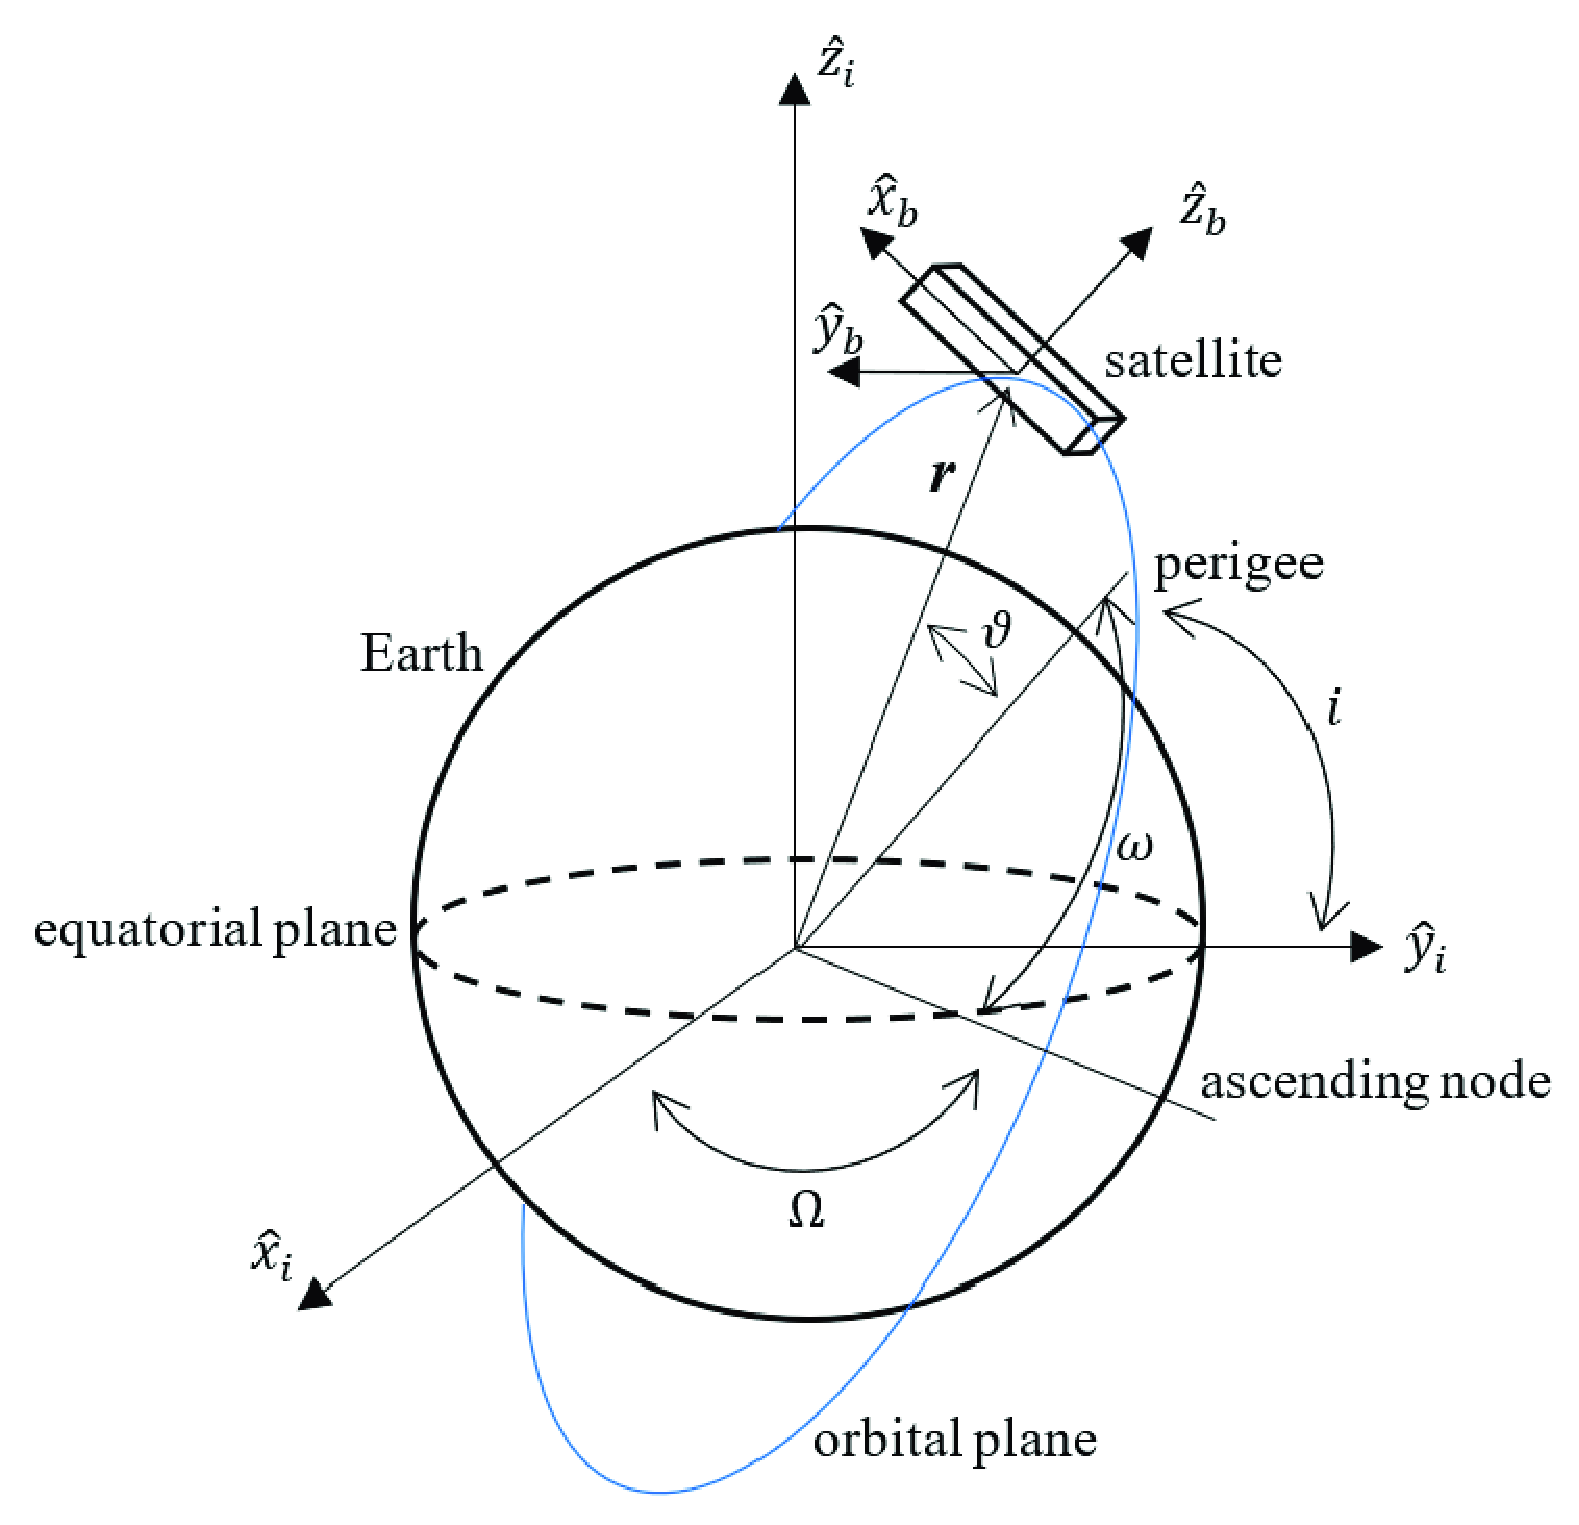
\includegraphics[width=0.85\textwidth]{gfx/gci.eps}
  \caption{\acrfull{gci} frame}
  \label{fig:raytracing}
\end{figure}

The chaser and target body-fixed frames have their origins at the \acrshort{cg} of both, respectively, and their axes are considered to be aligned with their respective principal axes. The origin of the camera frame instead coincides with the center of perspective projection. The target model frame is fixed with respect to the body frame and often coincides with it. For what concerns this work, for the sake of simplicity and without loss of generality, we will consider the camera frame to be coincident with the chaser body-fixed frame, and the target model frame to be coincident with the target body-fixed frame. 

\section{Image generation}
The use of artificial images gives a complete control over the scene. For the purpose of this work, a new procedure for the generation of realistic images, representative of a data-set taken by a monocular navigation camera during a close-proximity approach to target \acrshort{sc} has been developed.
Using the illustrated procedure, the user is able to create synthetic images of a target \acrshort{sc} given it's \acrshort{stl} model, by fine tuning all the properties of the materials composing the target \acrshort{sc}.
Since there could be also cases in which the Earth can be behind the target \acrshort{sc}, the developed tool is also able to simulate Earth's presence at any given location. The tool is also able to the simulate the the atmosphere of the Earth and the cloud layer \cite{jacopo}.
The developed tool couples the well known open-source raytracer \acrshort{povray} with MATLAB in order to archive a good degree of realism in the generated images.

\subsection{Ray Tracing}
Ray tracing is a rendering technique used for generating artificial images which relies on the concept of controlling the path of view lines which starts from the observer camera and ends to generic virtual objects and thus calculating the color intensity of the object.
What is really of crucial importance for our particular use case is that ray tracing is capable of re-creating some of nature's optical effects through transparent and opaque surfaces as reflection and refraction, scattering, and dispersion phenomena (such as chromatic aberration).
Due to this, ray tracing techniques can generate artificial images with a really high degree of photorealism.
When the ray tracer renders the scene, a ray of light is traced for every pixel of the camera. Typically, each ray must be tested for intersection with some subset of the objects in the scene. Once the ray has intercepted an object, the ray tracing algorithm will estimate the amount and the type of incoming light at the point of intersection, examine the material properties and by combining those information will calculate the final color intensity that should be attributed to the pixel.
Several illumination algorithms and reflective or translucent materials may also require more rays to be re-cast into the scene in order to do the necessary computations.
At first glance may seem cumbersome to start the ray from the observer towards the object rather than casting rays to the camera (as is in reality). However, doing so speeds up a lot the computation time, as most of the light rays present in a scene may never reach the eye of the observer, and so, all the time spent for tracing those would be useless.
After either a maximum number of reflections or a ray traveling a certain distance without intersection, the ray ceases to travel and the pixel's value is updated.

\begin{figure}[htbp]
  \centering
  \includegraphics[width=0.85\textwidth]{gfx/scherma-ray-tracing.eps}
  \caption{Raytracing: from the observer to the light source \cite{pictraytracing}}
  \label{fig:raytracing}
\end{figure}

For more information regarding how ray tracing works and ray tracing techniques in general, the interested reader can see \cite{introductionraytracing}.

\subsubsection{Ray tracing with \acrshort{povray}}
\acrshort{povray} is an open-source ray tracing software. It does not offer a GUI for modeling objects, but can be optionally used as Blender rendering engine in order to have a \acrshort{3d} modeling environment to model objects. \acrshort{povray} has also been already used to generate spaceborne imagery. For example, it has been used under the ESA LunarSim study to render images of lunar surfaces. Being an headless executable, \acrshort{povray} can be easily scripted in order to be used in conjunction with other softwares.
\acrshort{povray} gives the programmer several options to customize both the look and feel and the optical properties of the represented objects and the medium that light passes trough. \acrshort{povray} offers the choice to use some predefined geometric shapes, like spheres or cubes; another option instead is to define surfaces of the objects trough meshes. This capability has been used widely by this project to model the spacecraft object.
Any surface can then be characterized by its own optical properties. Every object can have a color specified by an Red Green Blue (RGB) triplet or can be wrapped with a texture.\\
For what concerns light sources, they have no visible shape of their own. They are just points or areas which emit light and can be tuned to accomplish the wanted result. For example we can tune the intensity of the light and the light color by specifying the RGB triplet; any atmospheric effect like opaque gas presence (like smoke or clouds) and its relative optical distortions can be modeled as well.

\subsection{Environment Modeling}
\subsubsection{Earth Modeling}
Earth modeling has been developed in parallel to another thesis \cite{jacopo}.
Here will follow a brief review of how Earth has been modeled taken from \cite{jacopo}.
For modeling the Earth, the \acrshort{povray} \inlinecode{POV}{sphere} object has been used, in conjunction with the \inlinecode{POV}{scale} feature, which allows to make the sphere become an ellipsoid.

\begin{figure}[htbp]
  \centering
  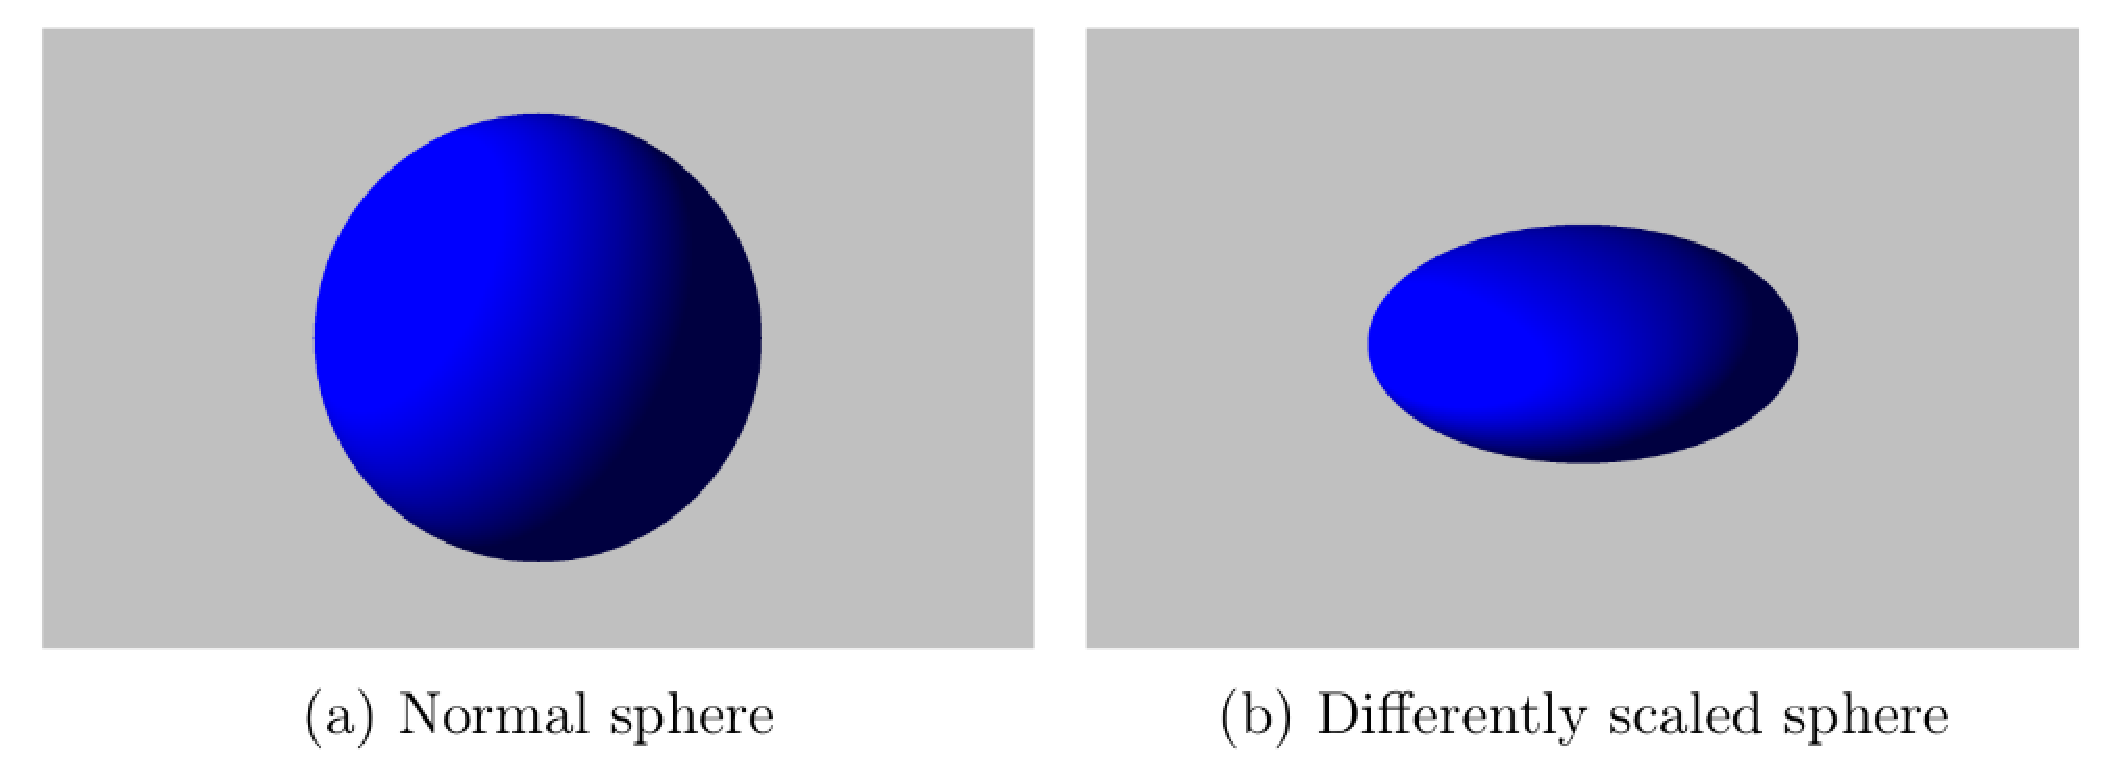
\includegraphics[width=0.85\textwidth]{gfx/sphere_scaling.eps}
  \caption{Sphere manipulation with \acrshort{povray} \cite{jacopo}}
  \label{fig:spherescaling}
\end{figure}

Once the \acrshort{3d} object is created, the most natural choice one can think of is to wrap a \acrshort{2d} texture of the Earth (figure \ref{fig:firstTexture}) on it, and this indeed is what has been done, using an high resolution texture of the Earth.

\begin{figure}[htbp]
  \centering
  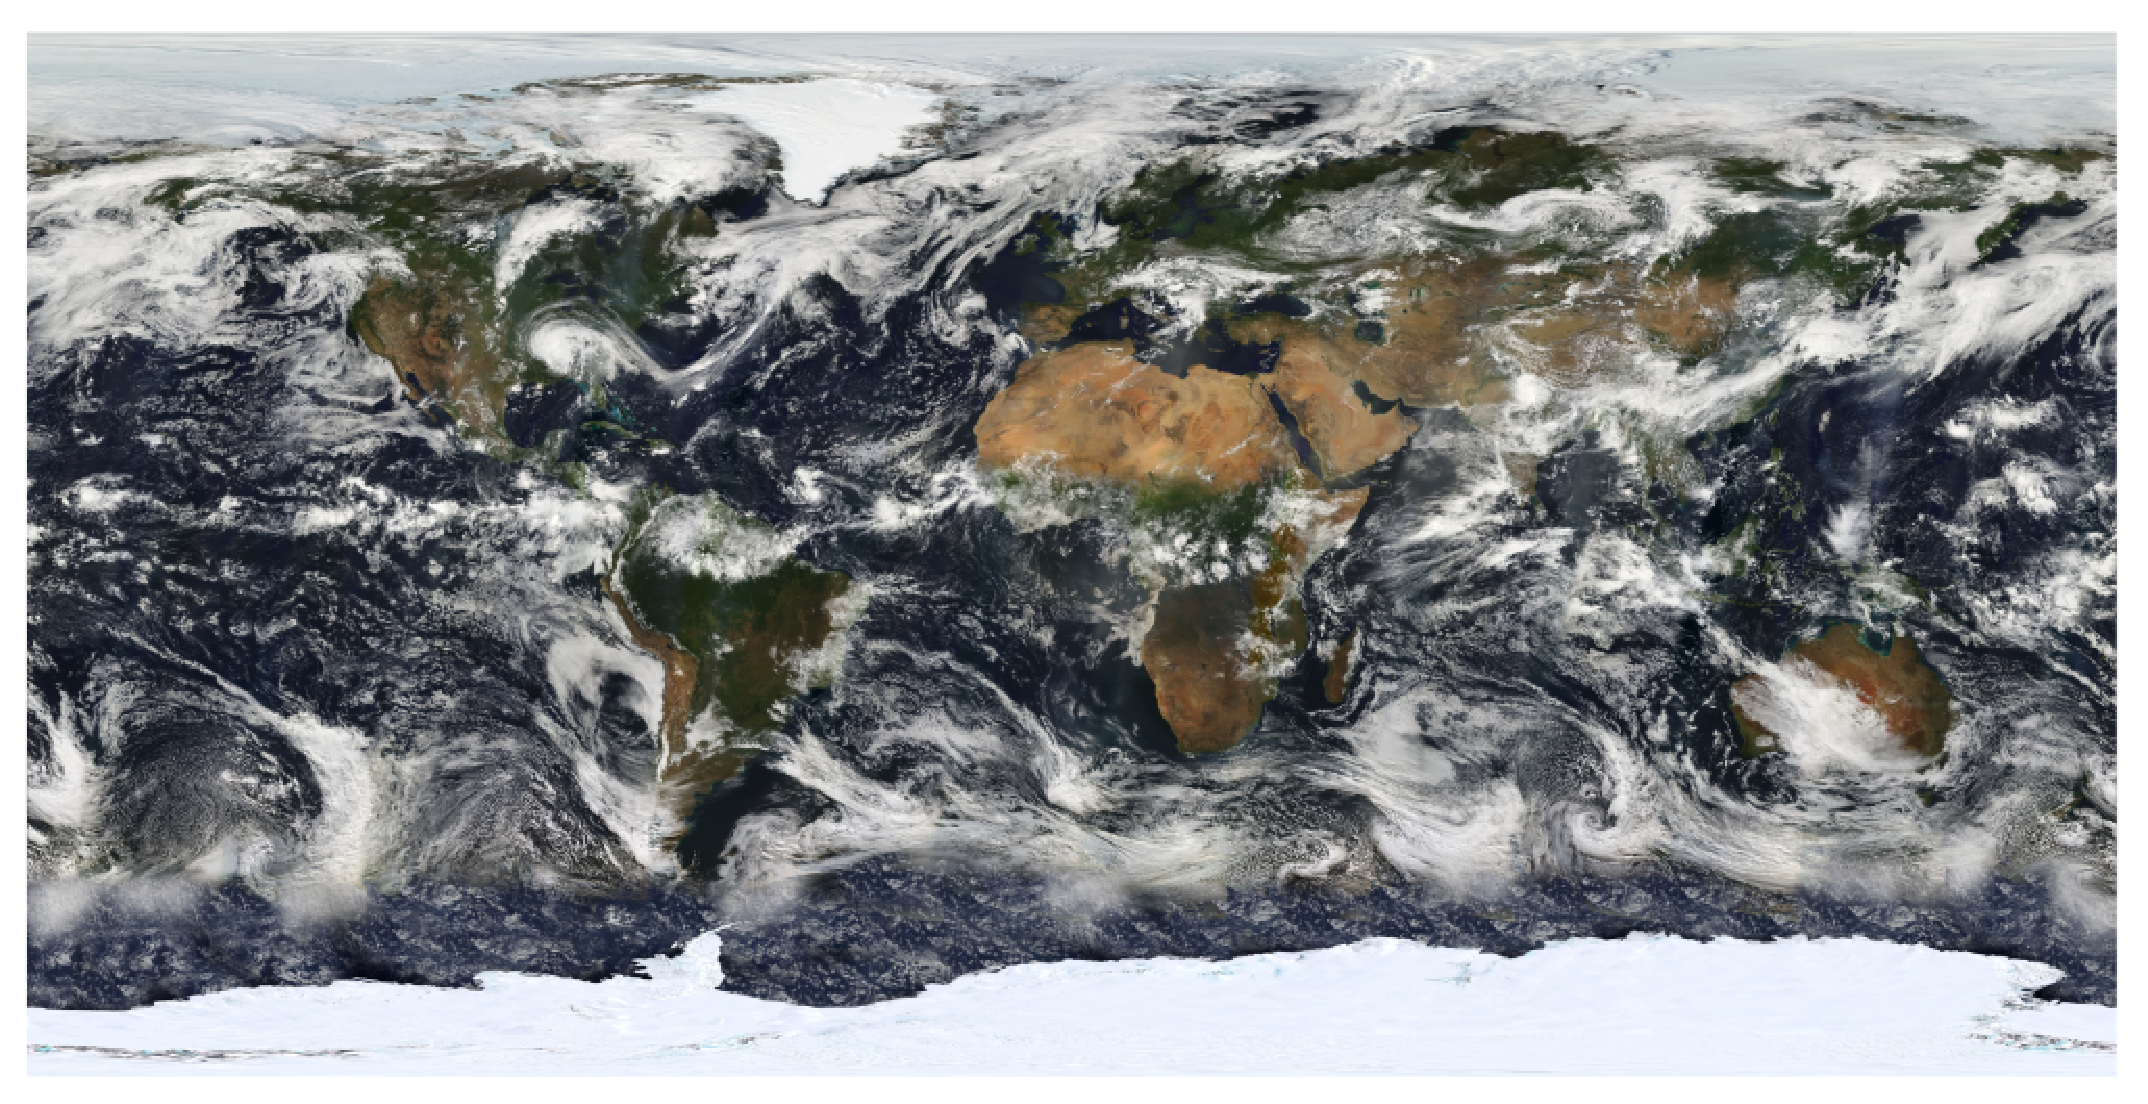
\includegraphics[width=0.85\textwidth]{gfx/first_text.eps}
  \caption{Initially chosen texture of the Earth}
  \label{fig:firstTexture}
\end{figure}

\bigskip

In figure \ref{fig:EarthApollo} we can see a comparison of the synthetically generated image and an actual true image of the Earth as seen from the Apollo 11. From a first glance, used texture gives a good representation of what we should see when we look of a picture of the Earth taken from the space.

\begin{figure}[htbp]
  \centering
  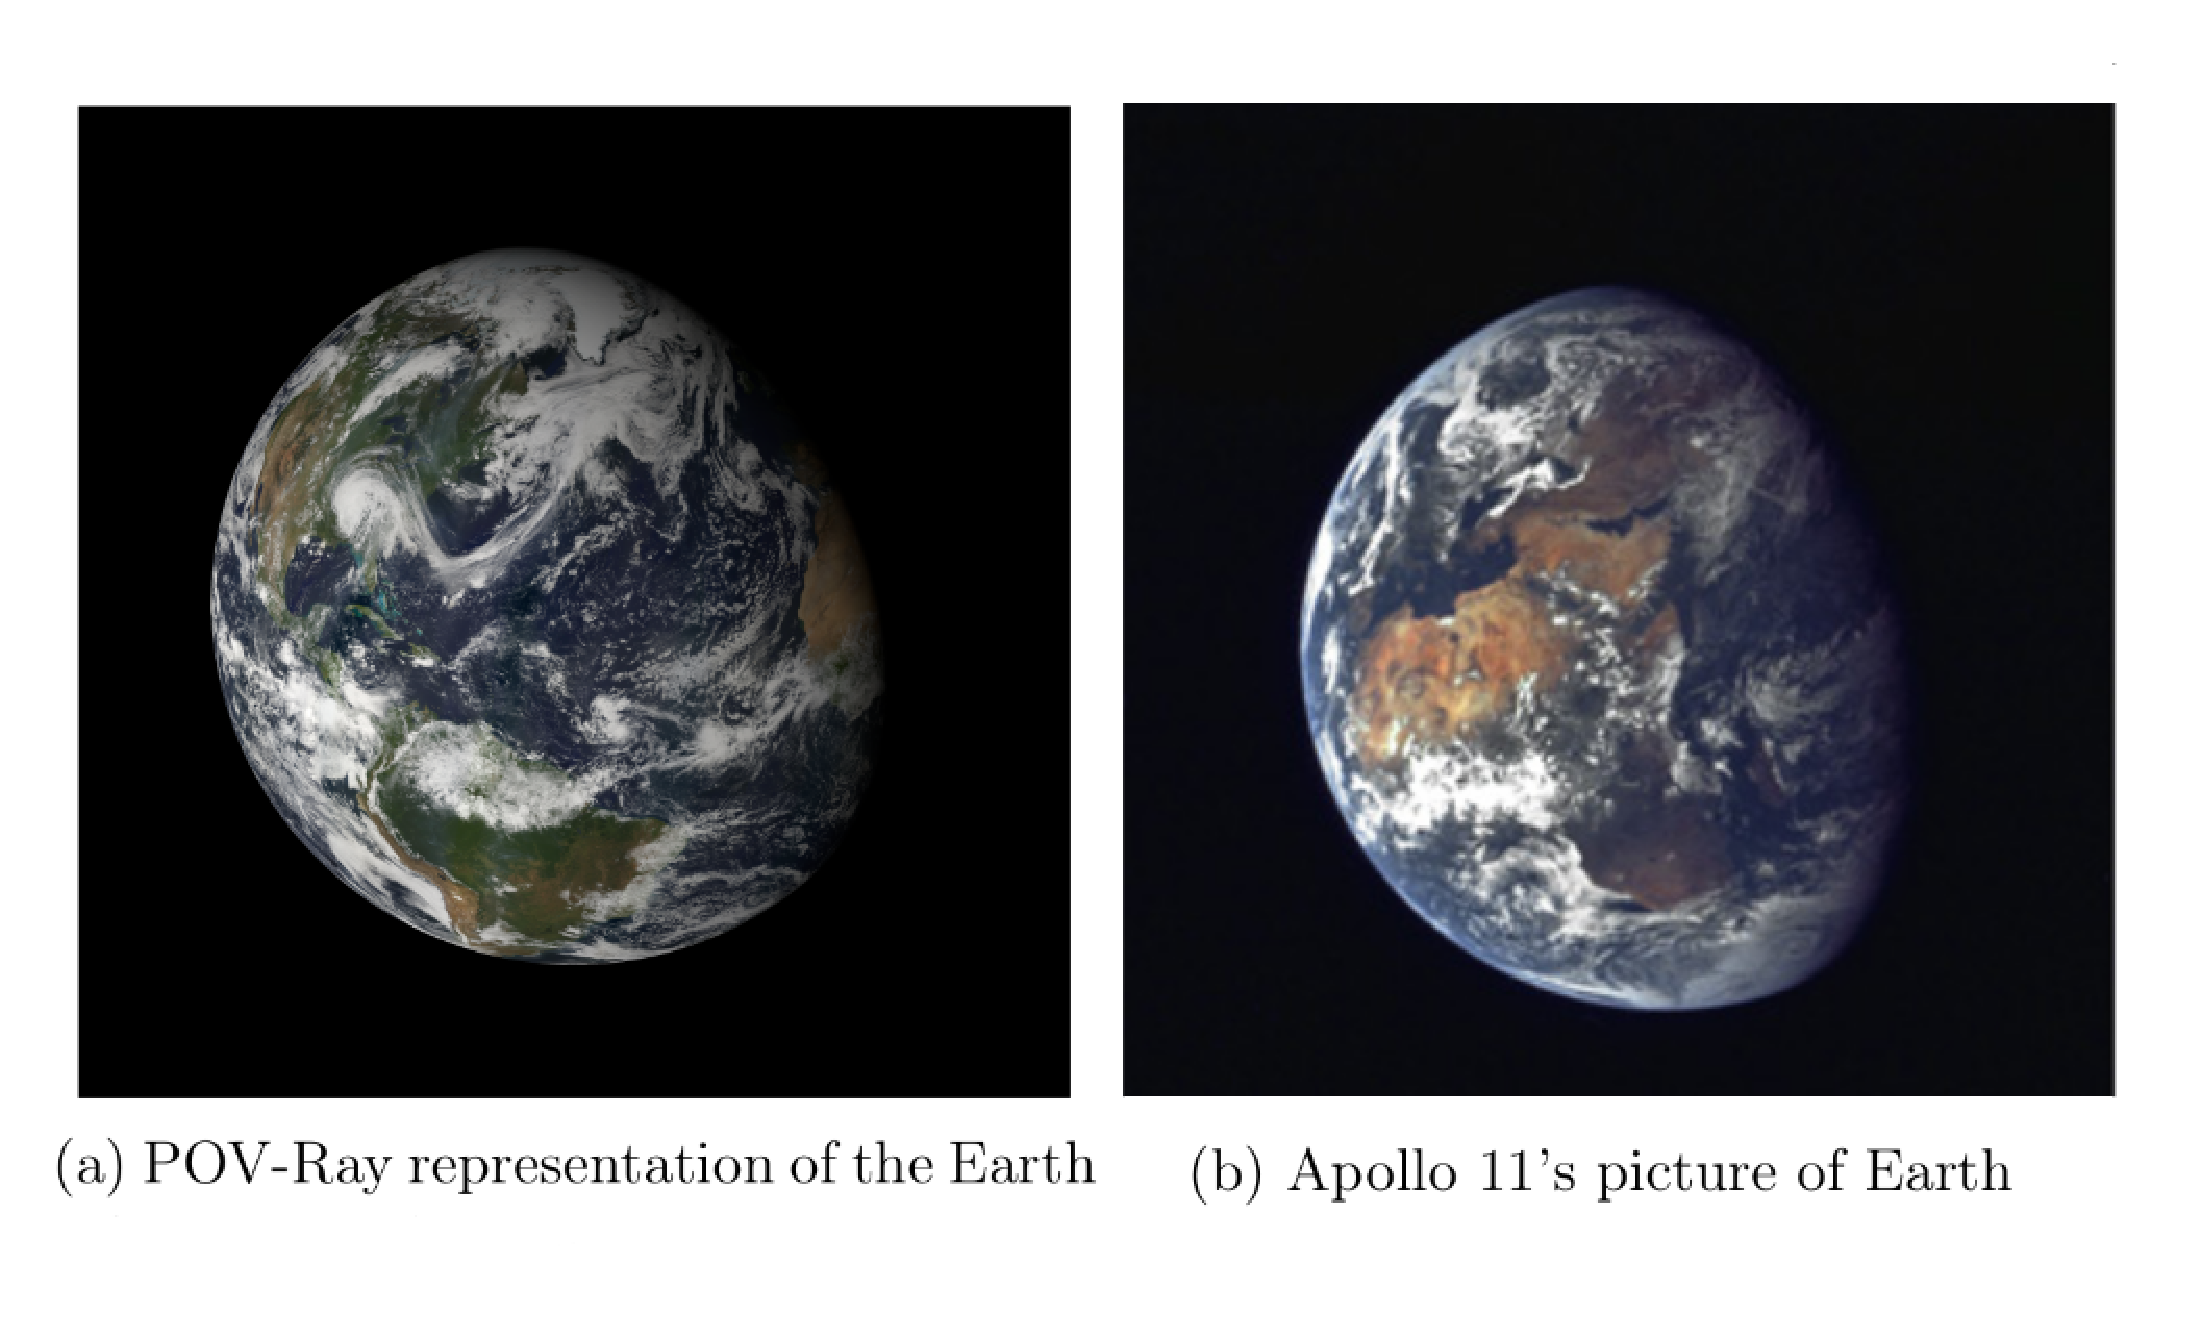
\includegraphics[width=0.85\textwidth]{gfx/earthApolloOurs.eps}
  \caption{Comparison of synthetic Earth image with Apollo 11's picture (the two images have different resolutions)}
  \label{fig:EarthApollo}
\end{figure}

Despite the relatively good result, this way of modeling the Earth still haves some issues :
\begin{itemize}
  \item since for all pictures we use the same texture, the clouds are sticked to their position on top of the surface of the Earth;
  \item terrains and seas are characterized by the same optical properties, while in reality they are not;
  \item diffusion of sunlight in the atmosphere is not simulated;
\end{itemize}
In the following paragraphs, those issues will be addressed.

\paragraph{Cloud Layer}\mbox{}\\
The fixed coupling of Earth surface and clouds is big problem for what concerns CV algorithms development, which should be trained to work in several different conditions, so, having the clouds always on the same region of the Earth despite the orientation is not acceptable.
The solution adopted in both this work and \cite{jacopo} relies on decoupling the Earth terrain layer and the cloud layer, specifying different optical properties for each layer, specify clouds relative rotation with respect to the terrain and coupling back everything together.
Furthermore, oceans have been split too, in order to be able to set different optical properties for the seas.
For the terrain layer, a a true-color mercator image of the Earth has been used as a base, in this way every piece of the surface could possibly be visible in any picture.

\begin{figure}[htbp]
  \centering
  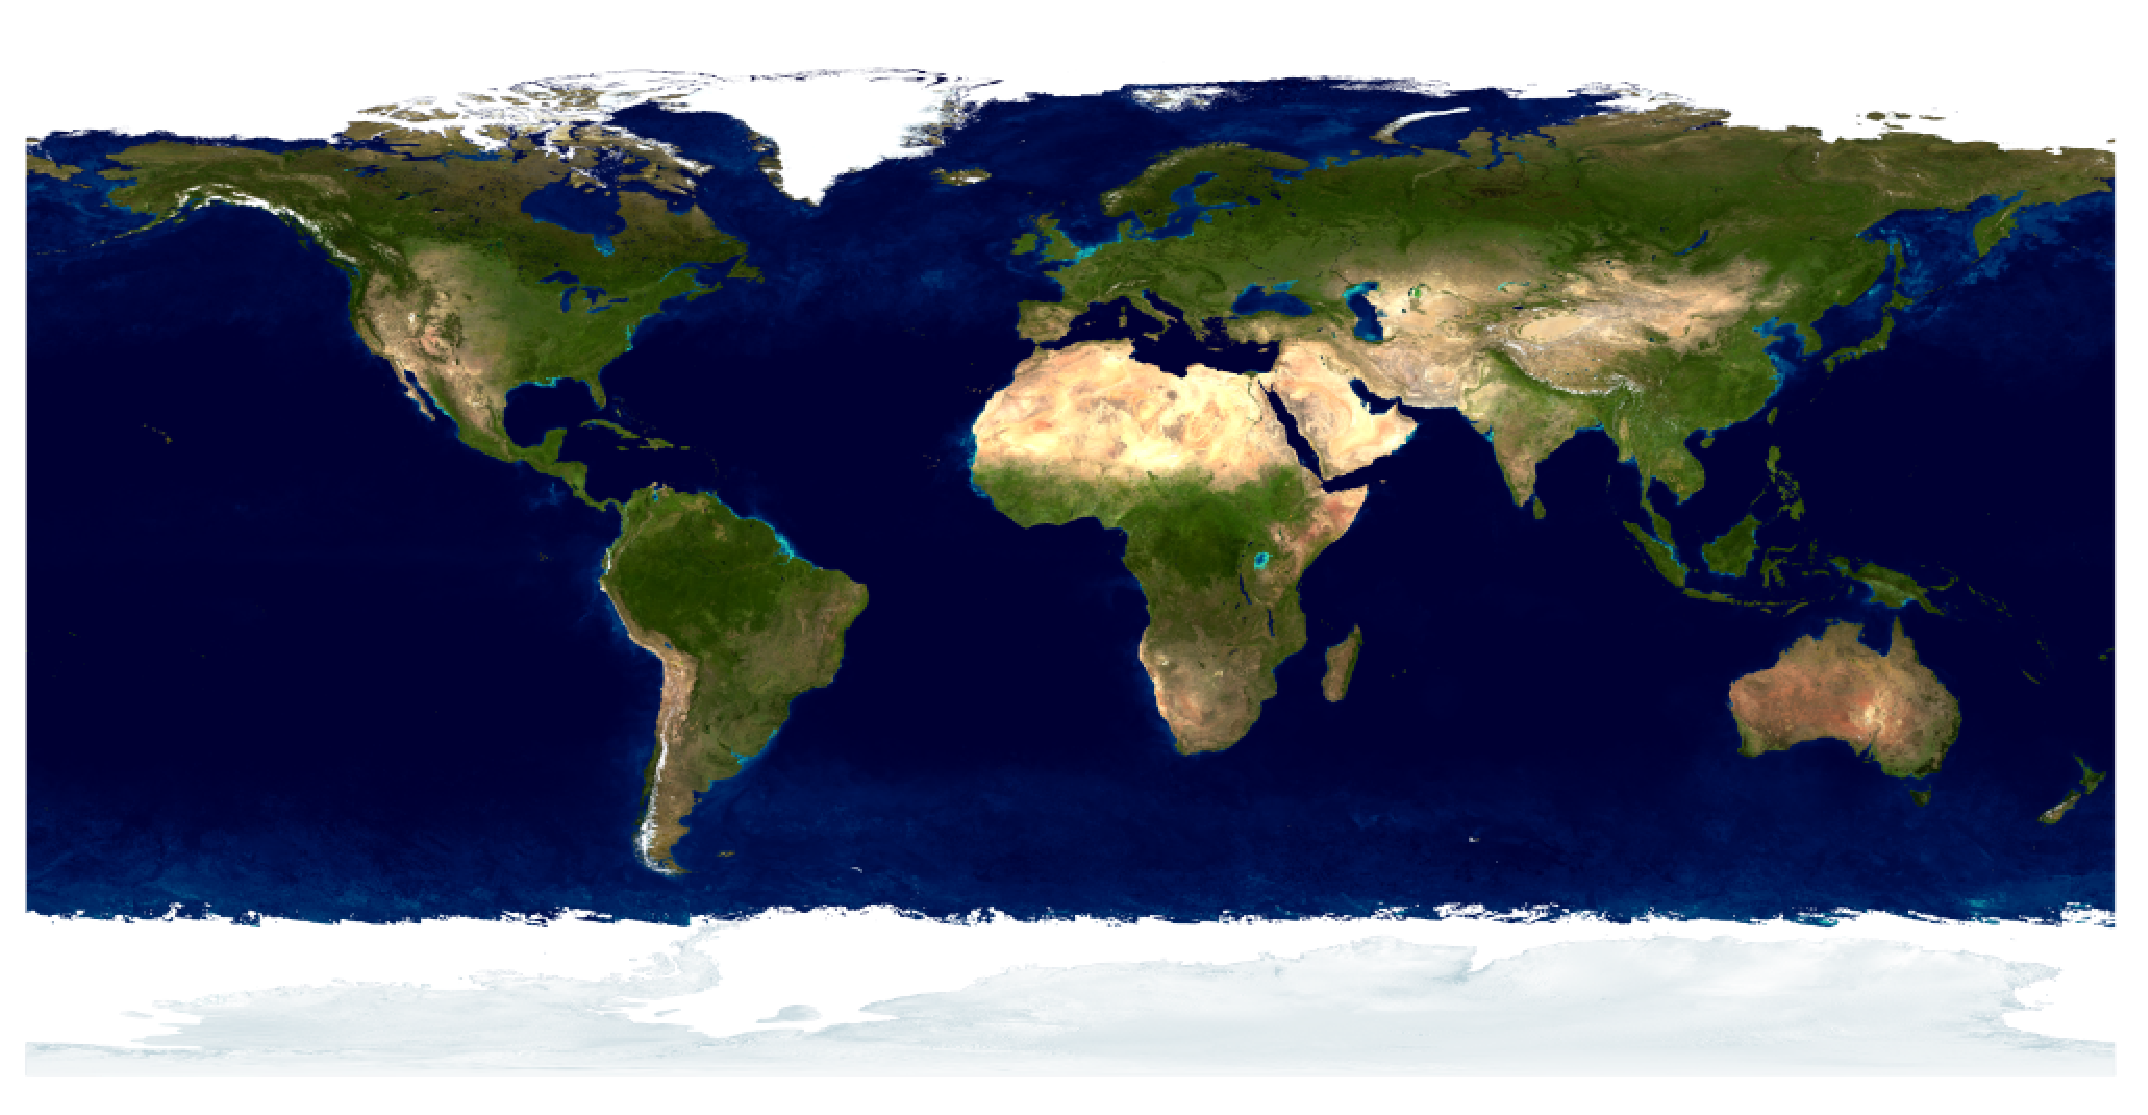
\includegraphics[width=0.85\textwidth]{gfx/earthMercator.eps}
  \caption{True Color Earth Mercator Image \cite{bluemarble}}
  \label{fig:EarthMercator}
\end{figure}

As said before, in order to be able to use different optical properties for water and terrains, a separate two-color mercator-projection image of the Earth where the water is black and the land is white has been used.

\begin{figure}[htbp]
  \centering
  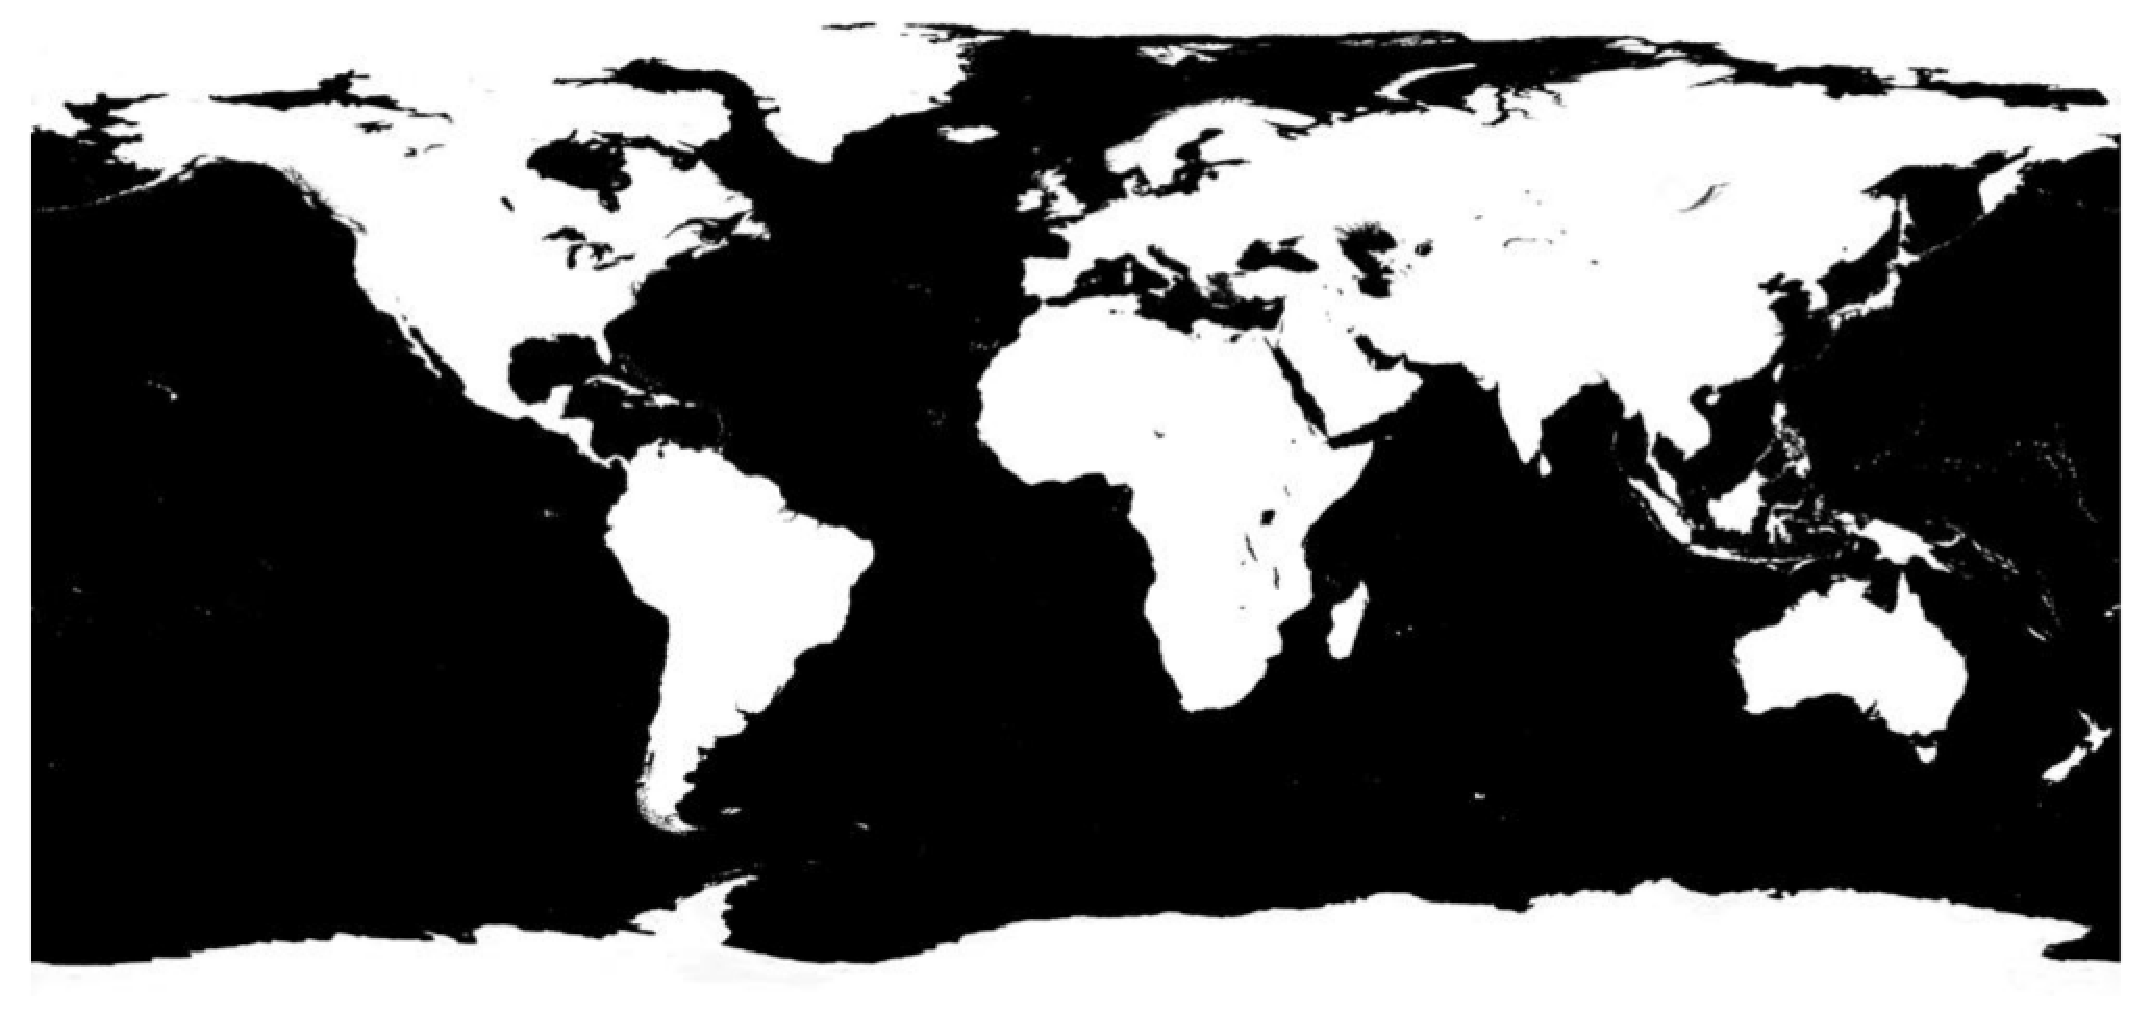
\includegraphics[width=0.85\textwidth]{gfx/landmask_mercator.eps}
  \caption{Landmask Mercator Image}
  \label{fig:LandmaskMercator}
\end{figure}

In figure \ref{fig:comparisonEarths} the result of differentiating the optical properties for terrains and oceans is shown. Despite the fact that it may seems that there is only a small distinction between the two images (in particular, shinier oceans and darker forests), is still enough the make the Earth to seem more photo-realistic, and it leave some space for further tuning.

\begin{figure}[htbp]
  \centering
  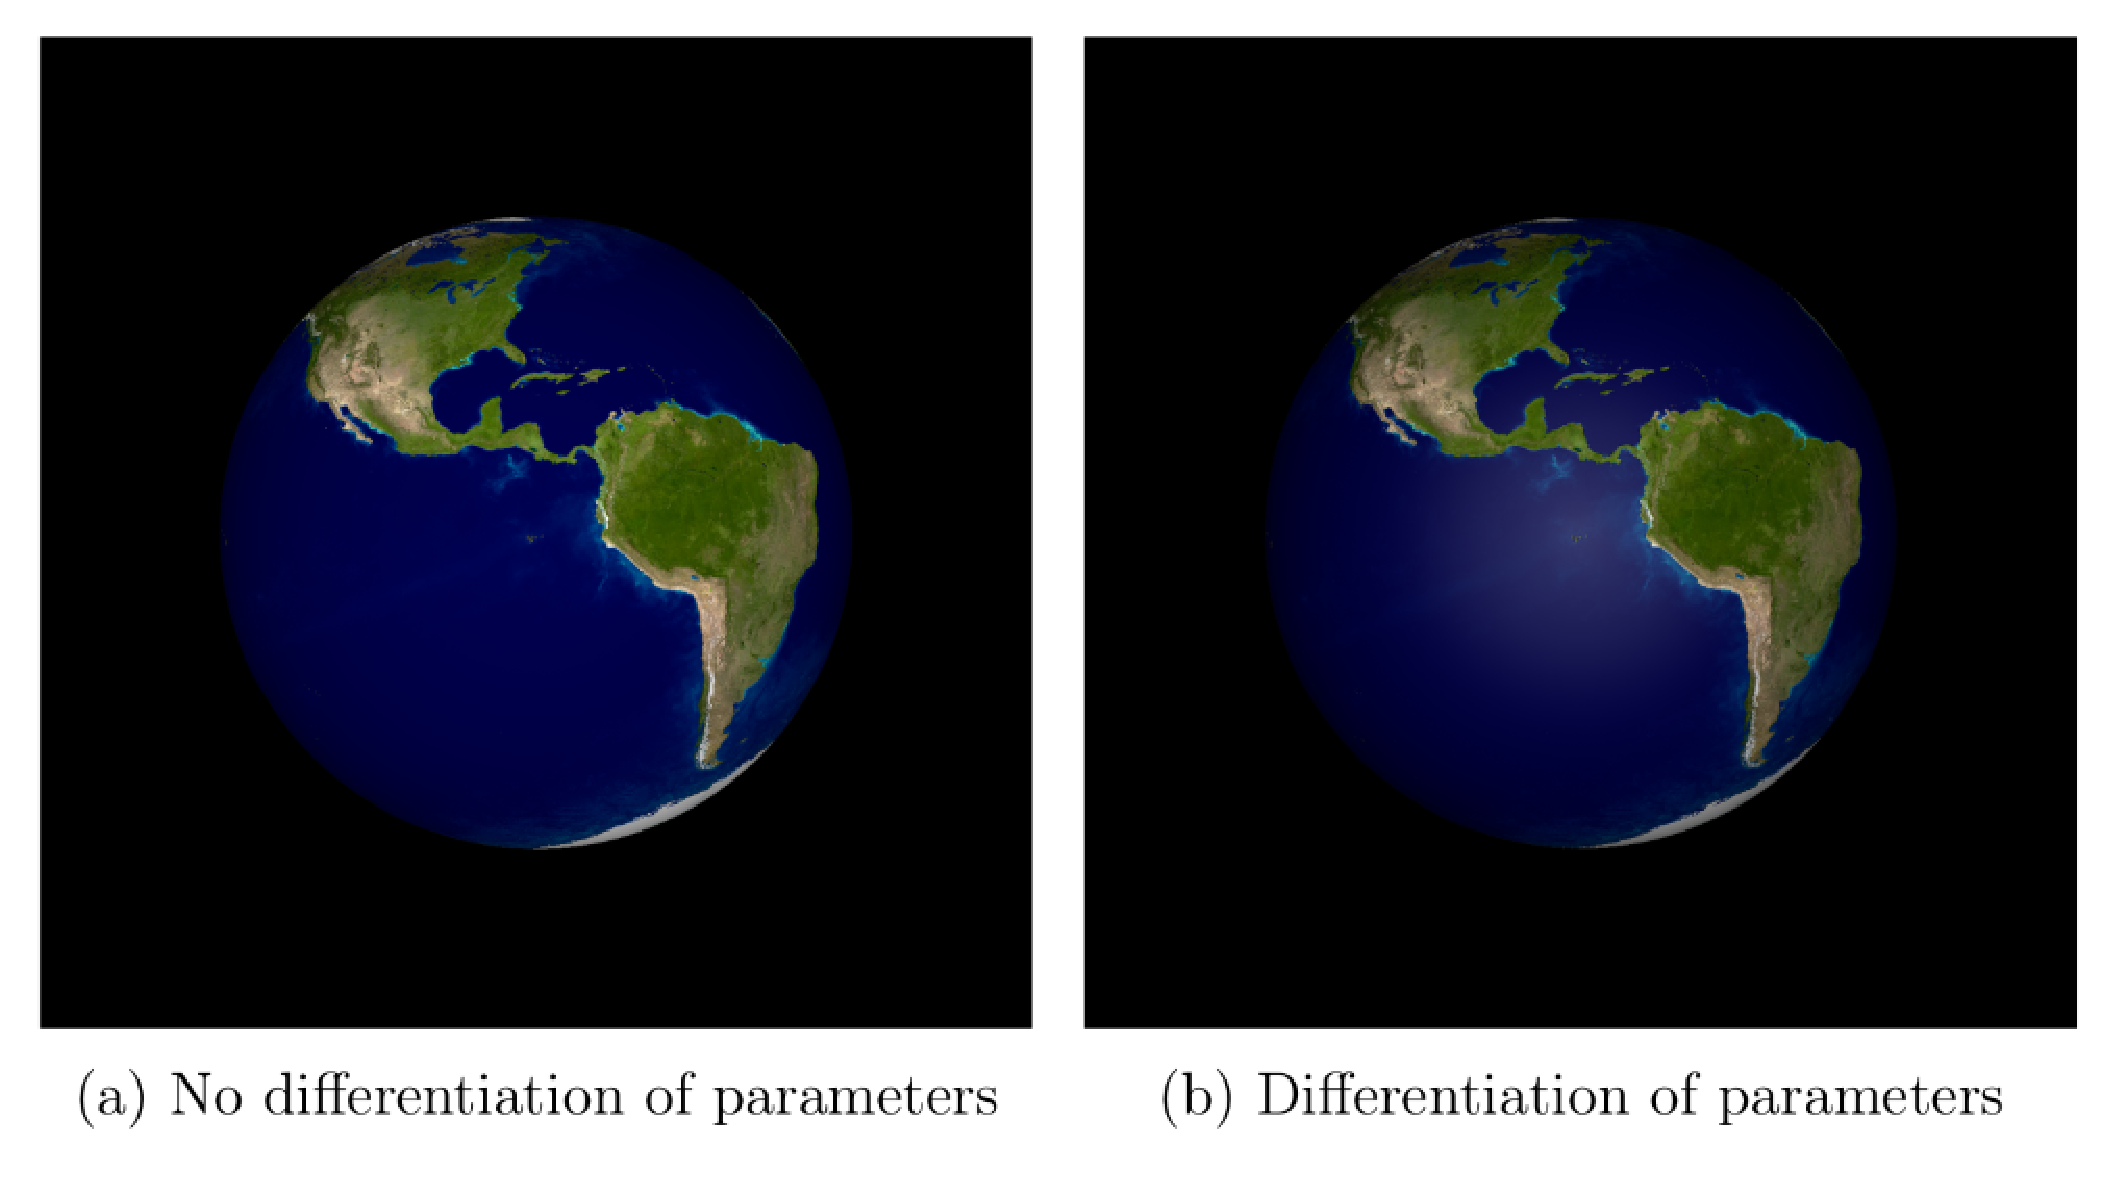
\includegraphics[width=0.82\textwidth]{gfx/comparisonEarths.eps}
  \caption{Comparing images with no differential treatment between land
    and ocean and with differential treatment}
  \label{fig:comparisonEarths}
\end{figure}

The cloud layer is added on top of the cloudless surface and thanks to that, it can rotate with respect to the Earth by a prescribed angle set by the programmer. The cloud layer texture and the shape of the clouds itself always remains the same, but this can be partially mitigated by using different cloud textures.

\begin{figure}[htbp]
  \centering
  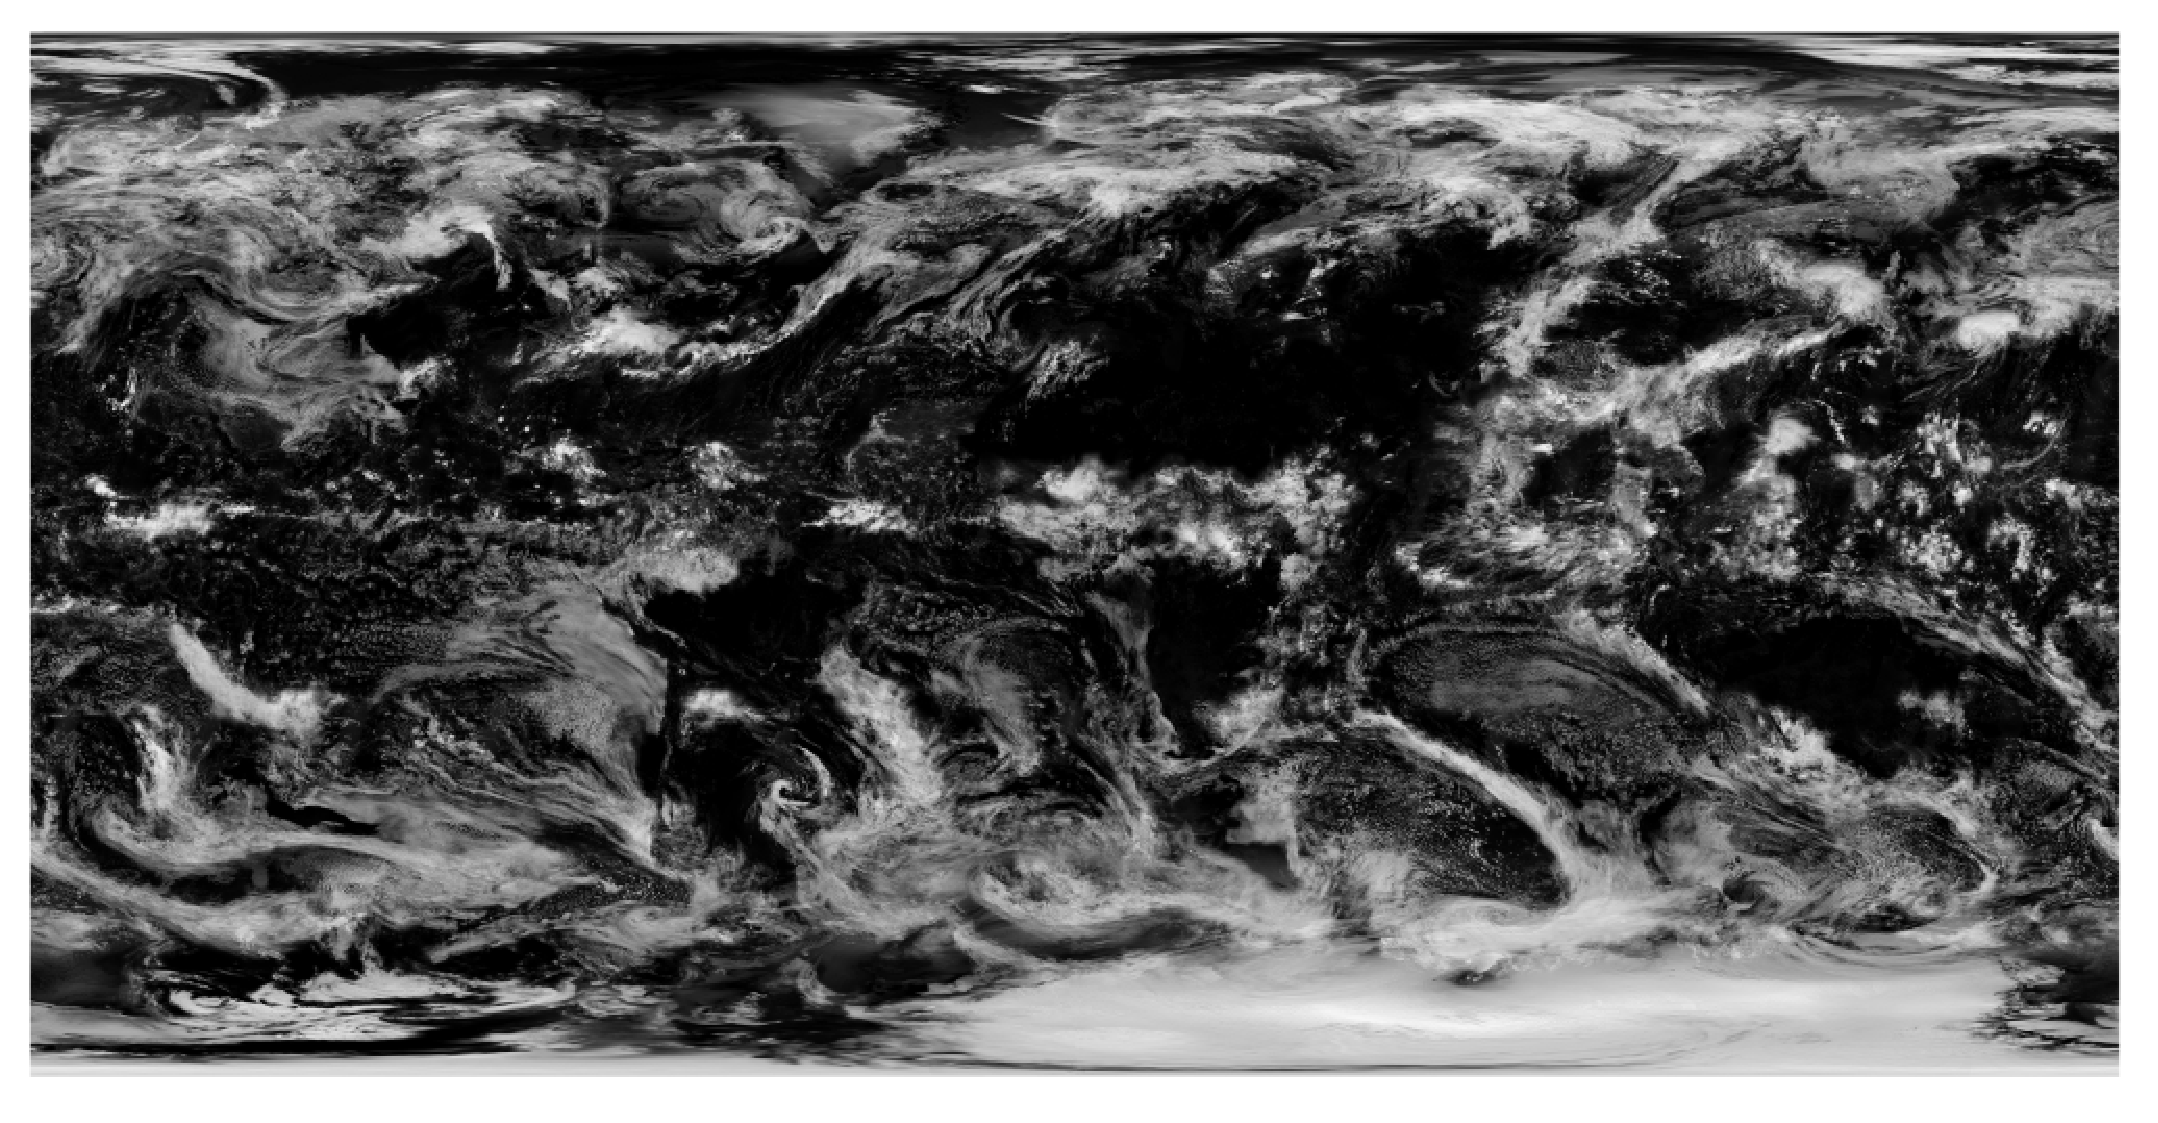
\includegraphics[width=0.85\textwidth]{gfx/clouds.eps}
  \caption{Two-color mercator image of Earth's cloud layer}
  \label{fig:cloudsMercator}
\end{figure}

The cloud texture used for this work (figure \ref{fig:cloudsMercator}) is not actually directly printed on the surface of the earth, but rather is extruded on a shell built around the sphere which defines the Earth, which has an inner radius equal to $R_{in} = 1.001 \cdot R_{Earth}$ and an outer radius equal to $R_{out} = 1.0002 \cdot  R_{Earth}$. Those values have been found by taking as a reference the fact that low Earth clouds ranges from an altitude of \SI{600}{\m} to \SI{15000}{\m} \cite{nimbostratus}. Although higher or thicker clouds can be modeled, this will require longer rendering times. Of course, also for the cloud layer is possible to set custom optical properties, in order to make the clouds partially transparent, so that when there isn't a dense cloud area, the terrain behind is still visible under the white blanket.\\
The result of adding the cloud layer can be seen in figure \ref{fig:cloudShell}

\begin{figure}[htbp]
  \centering
  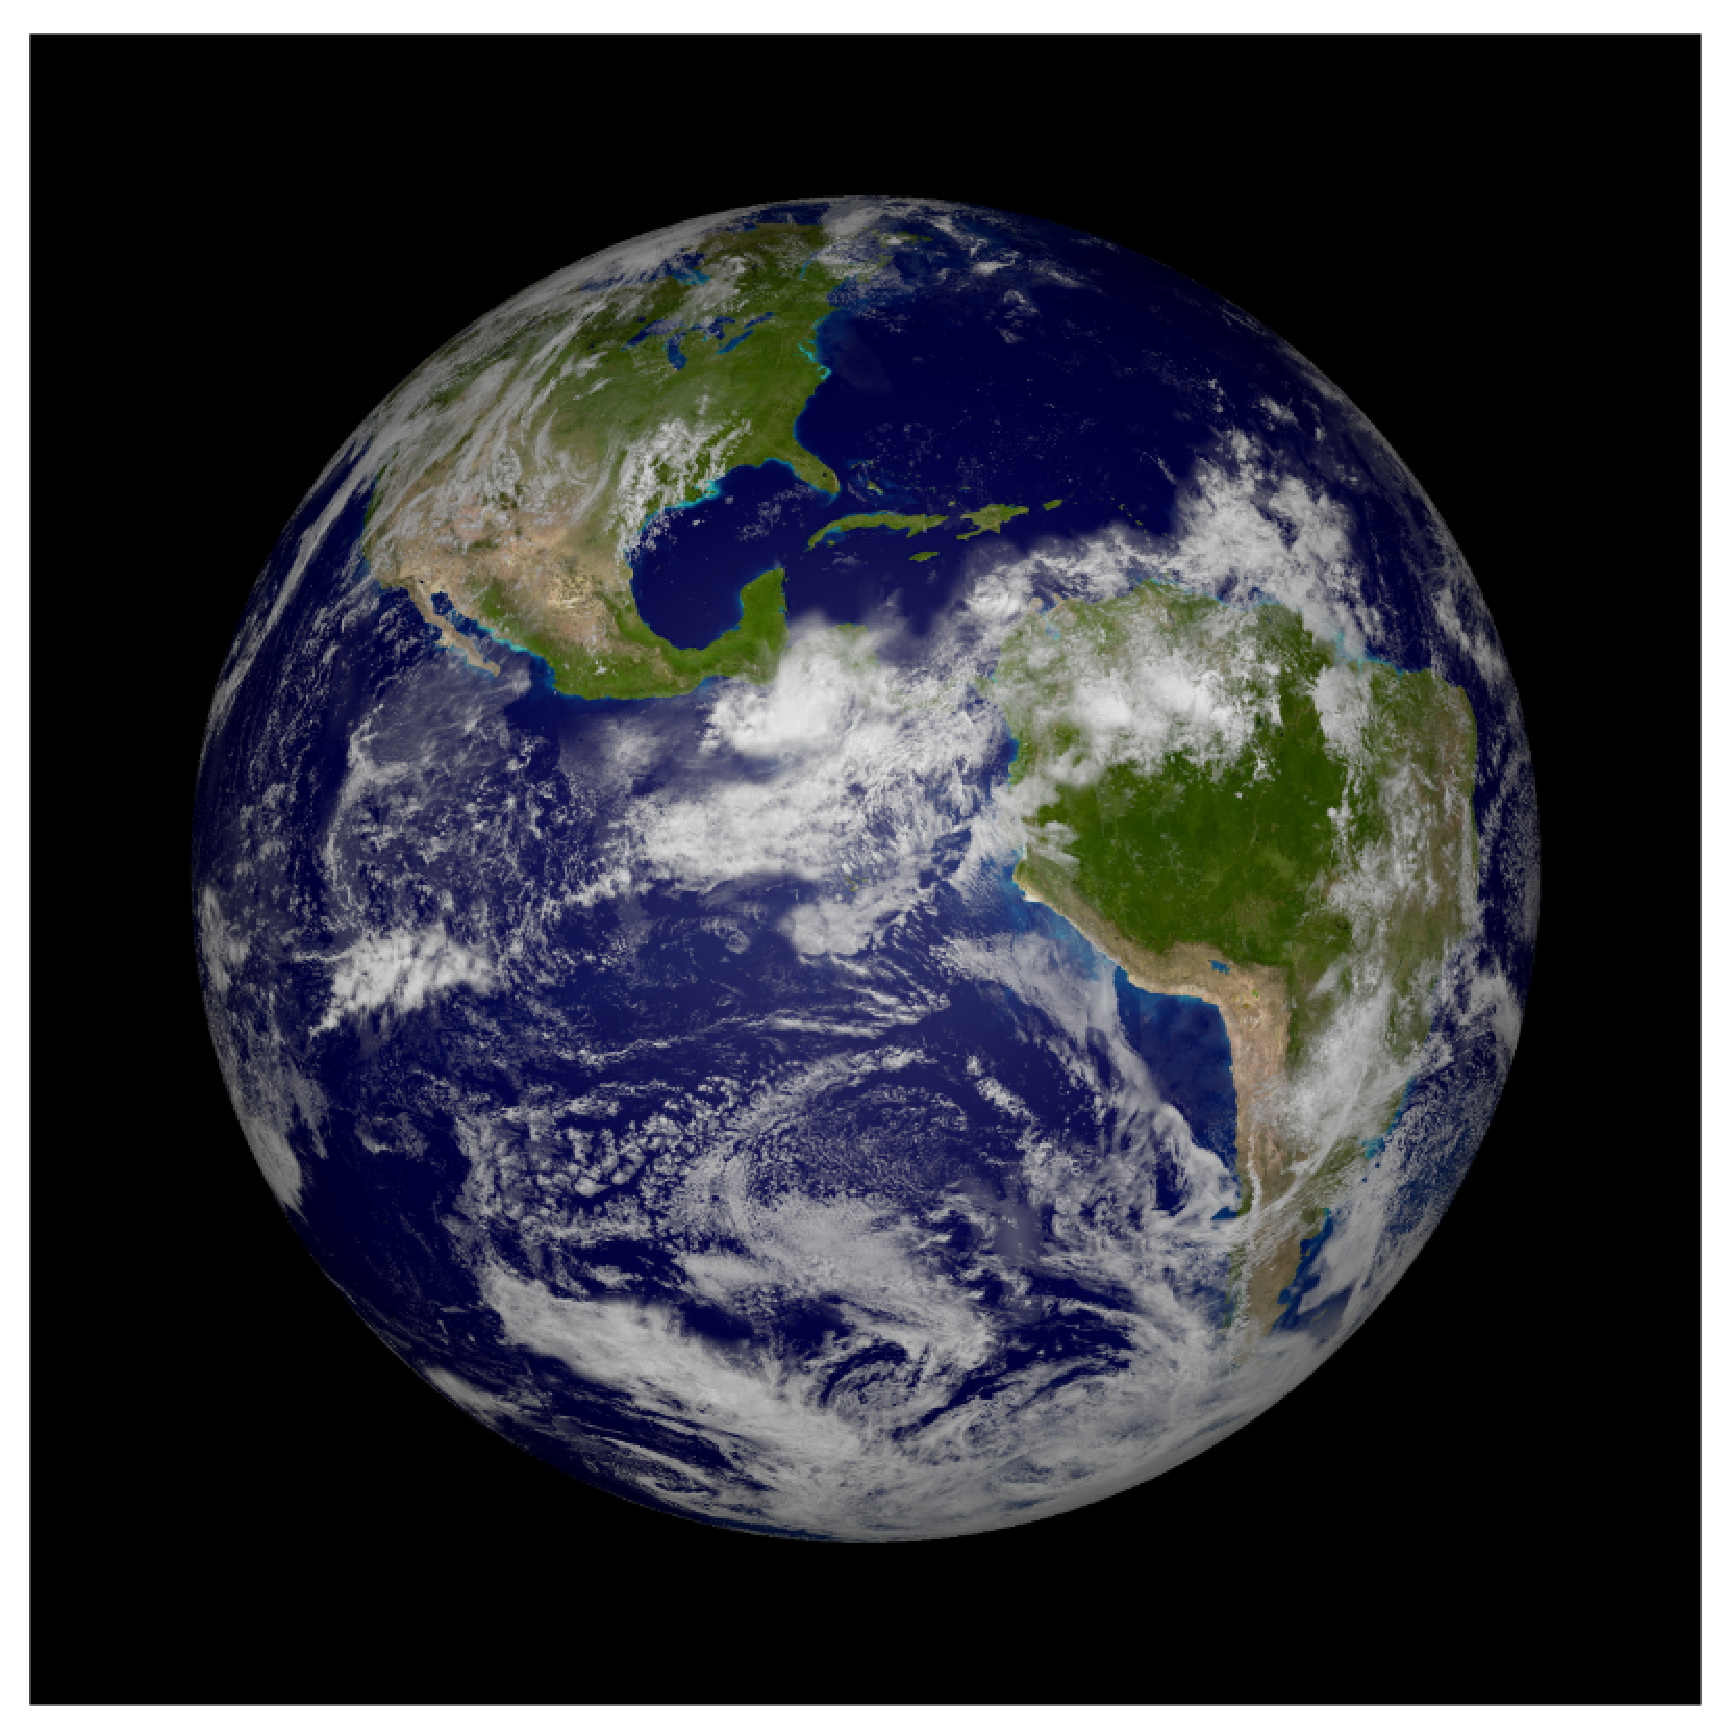
\includegraphics[width=0.72\textwidth]{gfx/cloudShell.eps}
  \caption{Earth's representation using cloud shell}
  \label{fig:cloudShell}
\end{figure}

\paragraph{Cloud Layer}\mbox{}\\
Recreating the characteristic atmosphere presence around the Earth is of crucial importance for developing a CV algorithm for space applications, as it is needed in order to train the algorithm itself to work into a real-case scenario.
The atmosphere's presence in fact would enlarge the aspect of the Earth in the image, and furthermore would stress the edge detection algorithms.
To recreate the atmospheric shine effect, a strategy which is similar to the one adopted to model the cloud layer has been used. In fact, it has been modeled as a shell with a certain thickness of a transparent material with some scattering properties.
For what concerns both this project and what has been done in \cite{jacopo}, the gaseous layer was made only \SI{25}{\km} thick. Despite the fact that the atmosphere should be visible up to many more kilometers, the computational load introduced by rendering a much high atmosphere is not negligible on a standard PC hardware, and so the image generation time would grow up exponentially, making the task of compiling a data-set of thousands of images very time consuming.
In figure \ref{fig:earthAtmo} can be seen the final result of adding the atmospheric model.

\begin{figure}[htbp]
  \centering
  \includegraphics[width=0.72\textwidth]{gfx/earthFinal.eps}
  \caption{Earth with the atmosphere layer}
  \label{fig:earthAtmo}
\end{figure}

In figure \ref{fig:trueVsFake} instead is possible to view the artificially generated next to a real Earth picture taken by NASA's Suomi NPP on January 4, 2012.
It can be seen that, despite the fact that the real image isn't perfectly reproduced (because some other factors should be known in order to be taken into account, such as exposure time), the synthetic image still provide an high degree of similarity with the real one.

\begin{figure}[htbp]
  \centering
  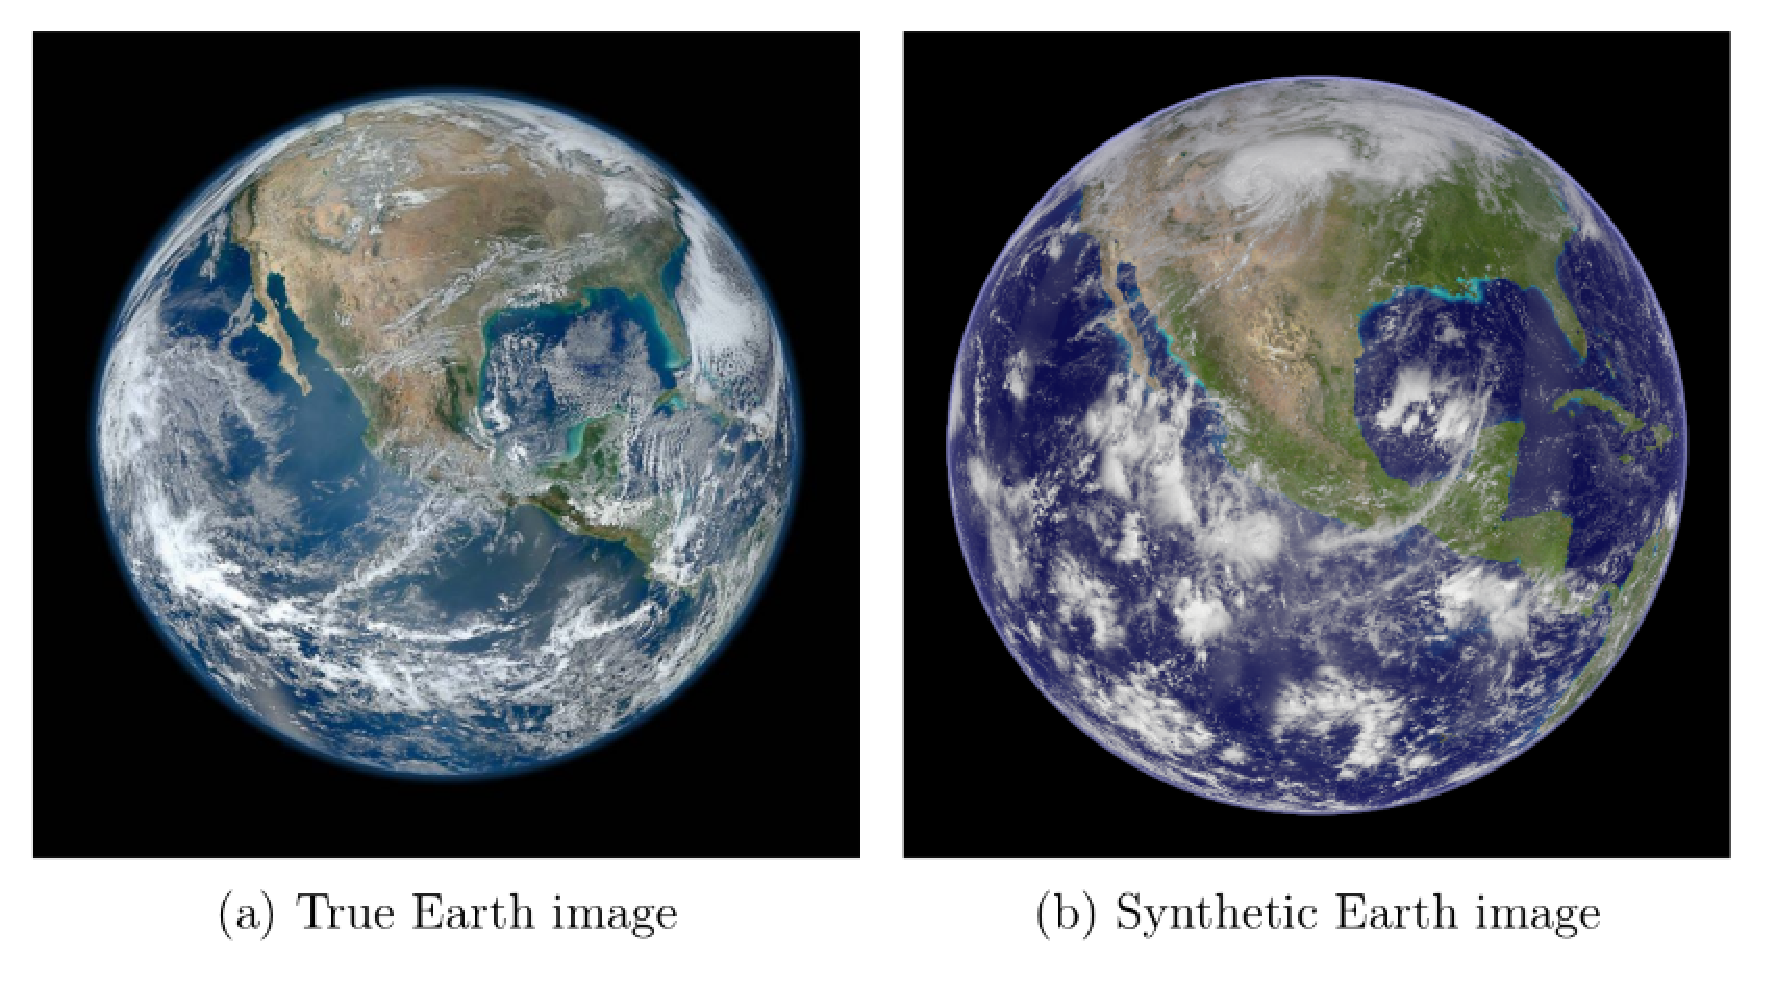
\includegraphics[width=1.0\textwidth]{gfx/trueVsFake.eps}
  \caption{Comparison between true \cite{bluemarble} and final rendered Earth image}
  \label{fig:trueVsFake}
\end{figure}

In table \ref{tab:EarthParameters} are briefly resumed the values used to model the various layer of the Earth.

\begin{table}[htbp]
  \centering
  \begin{tabular}{c cccc}
    \hline
    \hline
               & Terrain & Oceans       & Clouds & Atmosphere \\
    \hline
    Ambient    & 0.001   & 0.001        & 0.001  & 0.0001     \\
    Roughness  & 0.05    & 0.1          & 0.005  & 0.5        \\
    Brillance  & 1       & 1            & 1      & 1          \\
    Diffuse    & 0.85    & 0.85         & 1      & 0.6        \\
    Reflection & 0       & {0.04, 0.25} & 0      & 0          \\
    Specular   & 0       & 0.1          & 0      & 0          \\
    \hline
    \hline
  \end{tabular}
  \caption{Optical parameters of Earth's different layers}
  \label{tab:EarthParameters}
\end{table}

\subsubsection{Light Modeling}
For an object to show up into the scene, it must be illuminated.
There are two ways to illuminate an object with \acrshort{povray}:

\begin{itemize}
  \item use a standard light source
  \item use ambient light
\end{itemize}

The light source is controlled by the keyword \inlinecode{POV}{light_source}, which in turn accepts several modifiers. Light sources in \acrshort{povray}have no visible shape of their own. They are just points or areas which emit light.\\
The ambient light instead is controlled by the keyword \inlinecode{POV}{ambient} added to the \inlinecode{POV}{finish} modifier of an object, and it is used to simulate the light inside a shadowed area.
We can think of ambient light like a kind of light that is scattered everywhere in the room. It bounces all over the place and manages to light objects up a bit even where no light is directly shining.
In our particular case, we can use the \inlinecode{POV}{ambient} option to simulate the illumination of the object due to spurious light sources (such as stars) or reflection from other bodies (like the Moon or other planets).
In order to model the lightning condition of a true solar system, the light source has been modeled to resemble as much as possible the light emitted by the Sun.
The solution adopted in this project and in \cite{jacopo} relies upon modeling the sun as an area light source through the option \inlinecode{POV}{area_light}. This allows to create a cluster of point-like light sources distributed on a disc (simulated by adding the \inlinecode{POV}{circular} option to the area light source) which has radius equal to the radius of the Sun, and placed at the exact distance which the Sun has from the Earth in the \acrshort{gci} frame. In order to cope with the fact that in reality the Sun is equal to a sphere of light and not a disc, the option \inlinecode{POV}{orient} has been used. When using \inlinecode{POV}{orient}, every object in the \acrshort{povray} world would see the Sun's disc as oriented toward it, from any position around it.
Furthermore, the option \inlinecode{POV}{jitter} has been used, which tells the ray-tracer to slightly move the position of each light in the area light to eliminate any shadow banding that may occur.

\subsection{Spacecraft Modeling}

\subsubsection{3D Model of the Spacecraft}\label{sec:3dmodel}
The problem of modeling rather complex shapes with \acrshort{povray}, such as can be a spacecraft, it was one of the most demanding parts of this work, which also required to patch \acrshort{povray} source code, to prevent the ray tracer to forcibly use unnecessary features. Obviously, building the \acrshort{sc} using \acrshort{povray} primitives is a sub-optimal solution, as many different \acrshort{sc} can have different shapes, and modeling them by using simpler shapes each time it is simply not efficient. Furthermore, usually detaled \acrshort{3d} CAD models of \acrshort{sc} are available which can be easily exported into \acrshort{stl} format, so the focus has been putted into trying to understand how to translate those \acrshort{3d} CAD models directly into \acrshort{povray} code.
Several open source and closed source software have been coupled together in order to produce trough \acrshort{povray} a render of a given \acrshort{stl} model.
The procedure will be detailed in the following paragraphs.
The \acrshort{sc} which has been modeled for developing this thesis is heavily inspired by the Tango \acrshort{sc} of the PRISMA mission, by ESA.
The spacecraft has been modeled using the dimensions specified in \cite{Sharma2018}, which will be here reported for ease of reading. The solar panel is represented by a polygon of \SI{570}{\mm} x \SI{759}{\mm}, while the spacecraft body instead is represented by a convex polyhedron of \SI{560}{\mm} x \SI{550}{mm} x \SI{300}{\mm}. The radio frequency antennas length instead is of \SI{204}{\mm}. The origin of the CAD model is located in correspondence of the \acrshort{cg}.\\
Using the aforementioned dimensions, the Tango spacecraft has firstly been reproduced using Autodesk Inventor. The result of the modeling procedure is shown in figure \ref{fig:tango3d}.

\begin{figure}[htbp]
  \centering
  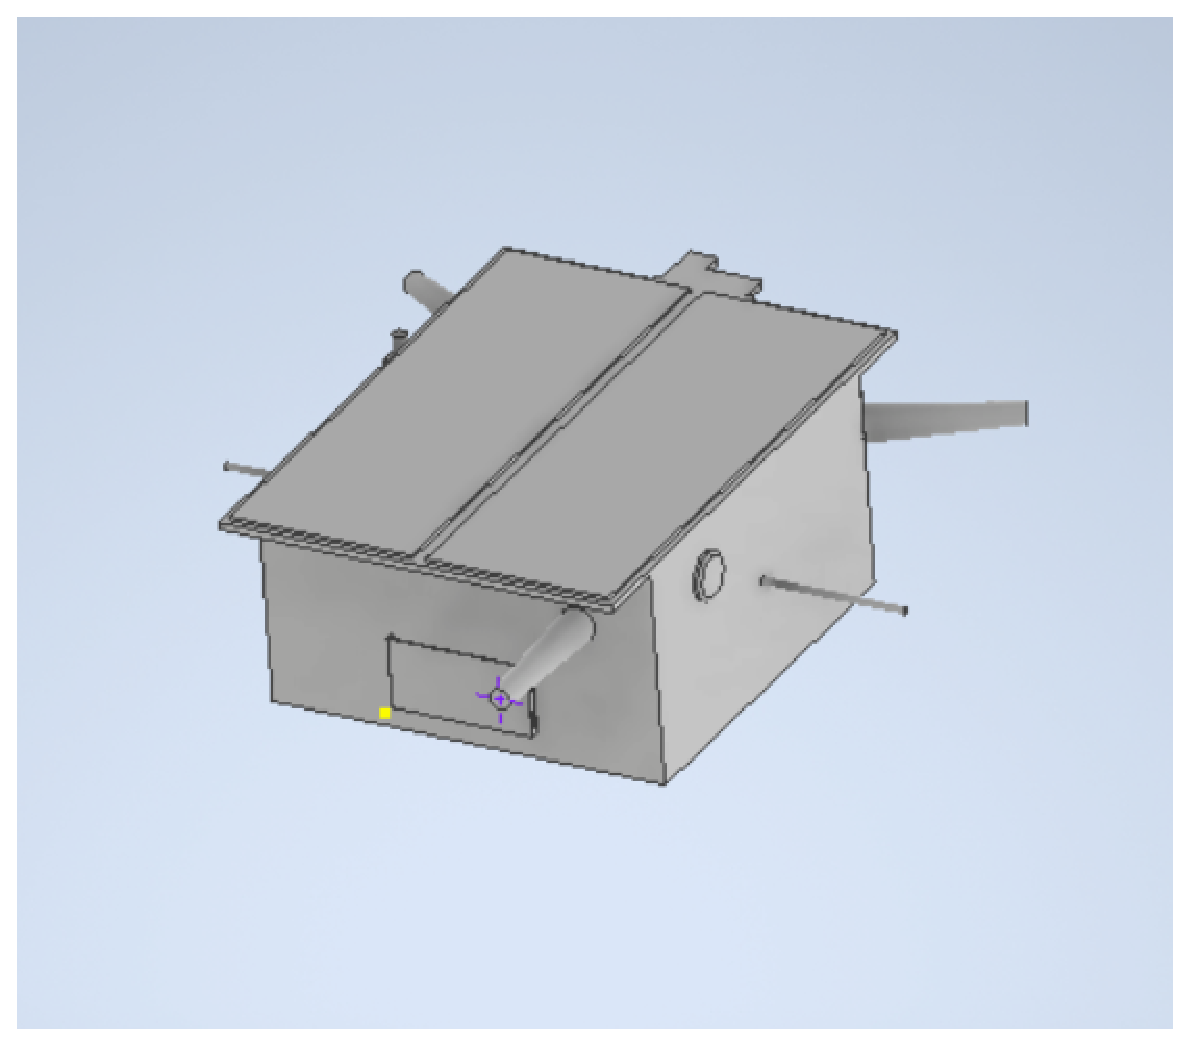
\includegraphics[width=0.62\textwidth]{gfx/tangoScreenshot2.eps}
  \caption{Tango \acrshort{sc} \acrshort{3d} model}
  \label{fig:tango3d}
\end{figure}
The \acrshort{3d} CAD model can now be exported in \acrshort{stl} format to be manipulated through other software.

\subsubsection{Blender}
Once the \acrshort{3d} model of the Tango \acrshort{sc} was available, the most challenging task has been the one of rendering the \acrshort{sc} itself using \acrshort{povray} at attitudes imposed by the user.
The first step for archiving that goal is to import the \acrshort{stl} model of the \acrshort{sc} into Blender. By exploiting the \acrshort{povray} render add-on for Blender, it is possible to render any given \acrshort{stl} file imported file using \acrshort{povray} as rendering engine. The \acrshort{povray} add-on will optionally save the generated SDL code used to render the scene.
The generated code however, will threat the entire \acrshort{3d} model as a whole, generating one giant \acrshort{povray} \inlinecode{POV}{mesh2} object, that is something which cannot be easily managed. Just as an example, would be impossible to assign to the different parts of the \acrshort{sc} different optical parameters or textures.
So, to workaround this limitation, it is a good practice to first split the different surfaces of the \acrshort{3d} model in different different children objects (or children surfaces), and only after render the scene in order to get the POV code. In this way, the \acrshort{povray} render add-on for Blender will generate a \textbf{mesh2} object for each children object created in Blender.
This will enable us to set different material properties for each children surface or to apply different textures to different surfaces.
For the purpose of this work, the original \acrshort{stl} model has been subdivided into thirty children object, each one with its own optical parameters, as can be seen from figure \ref{fig:tangoblender} .

\begin{figure}[htbp]
  \centering
  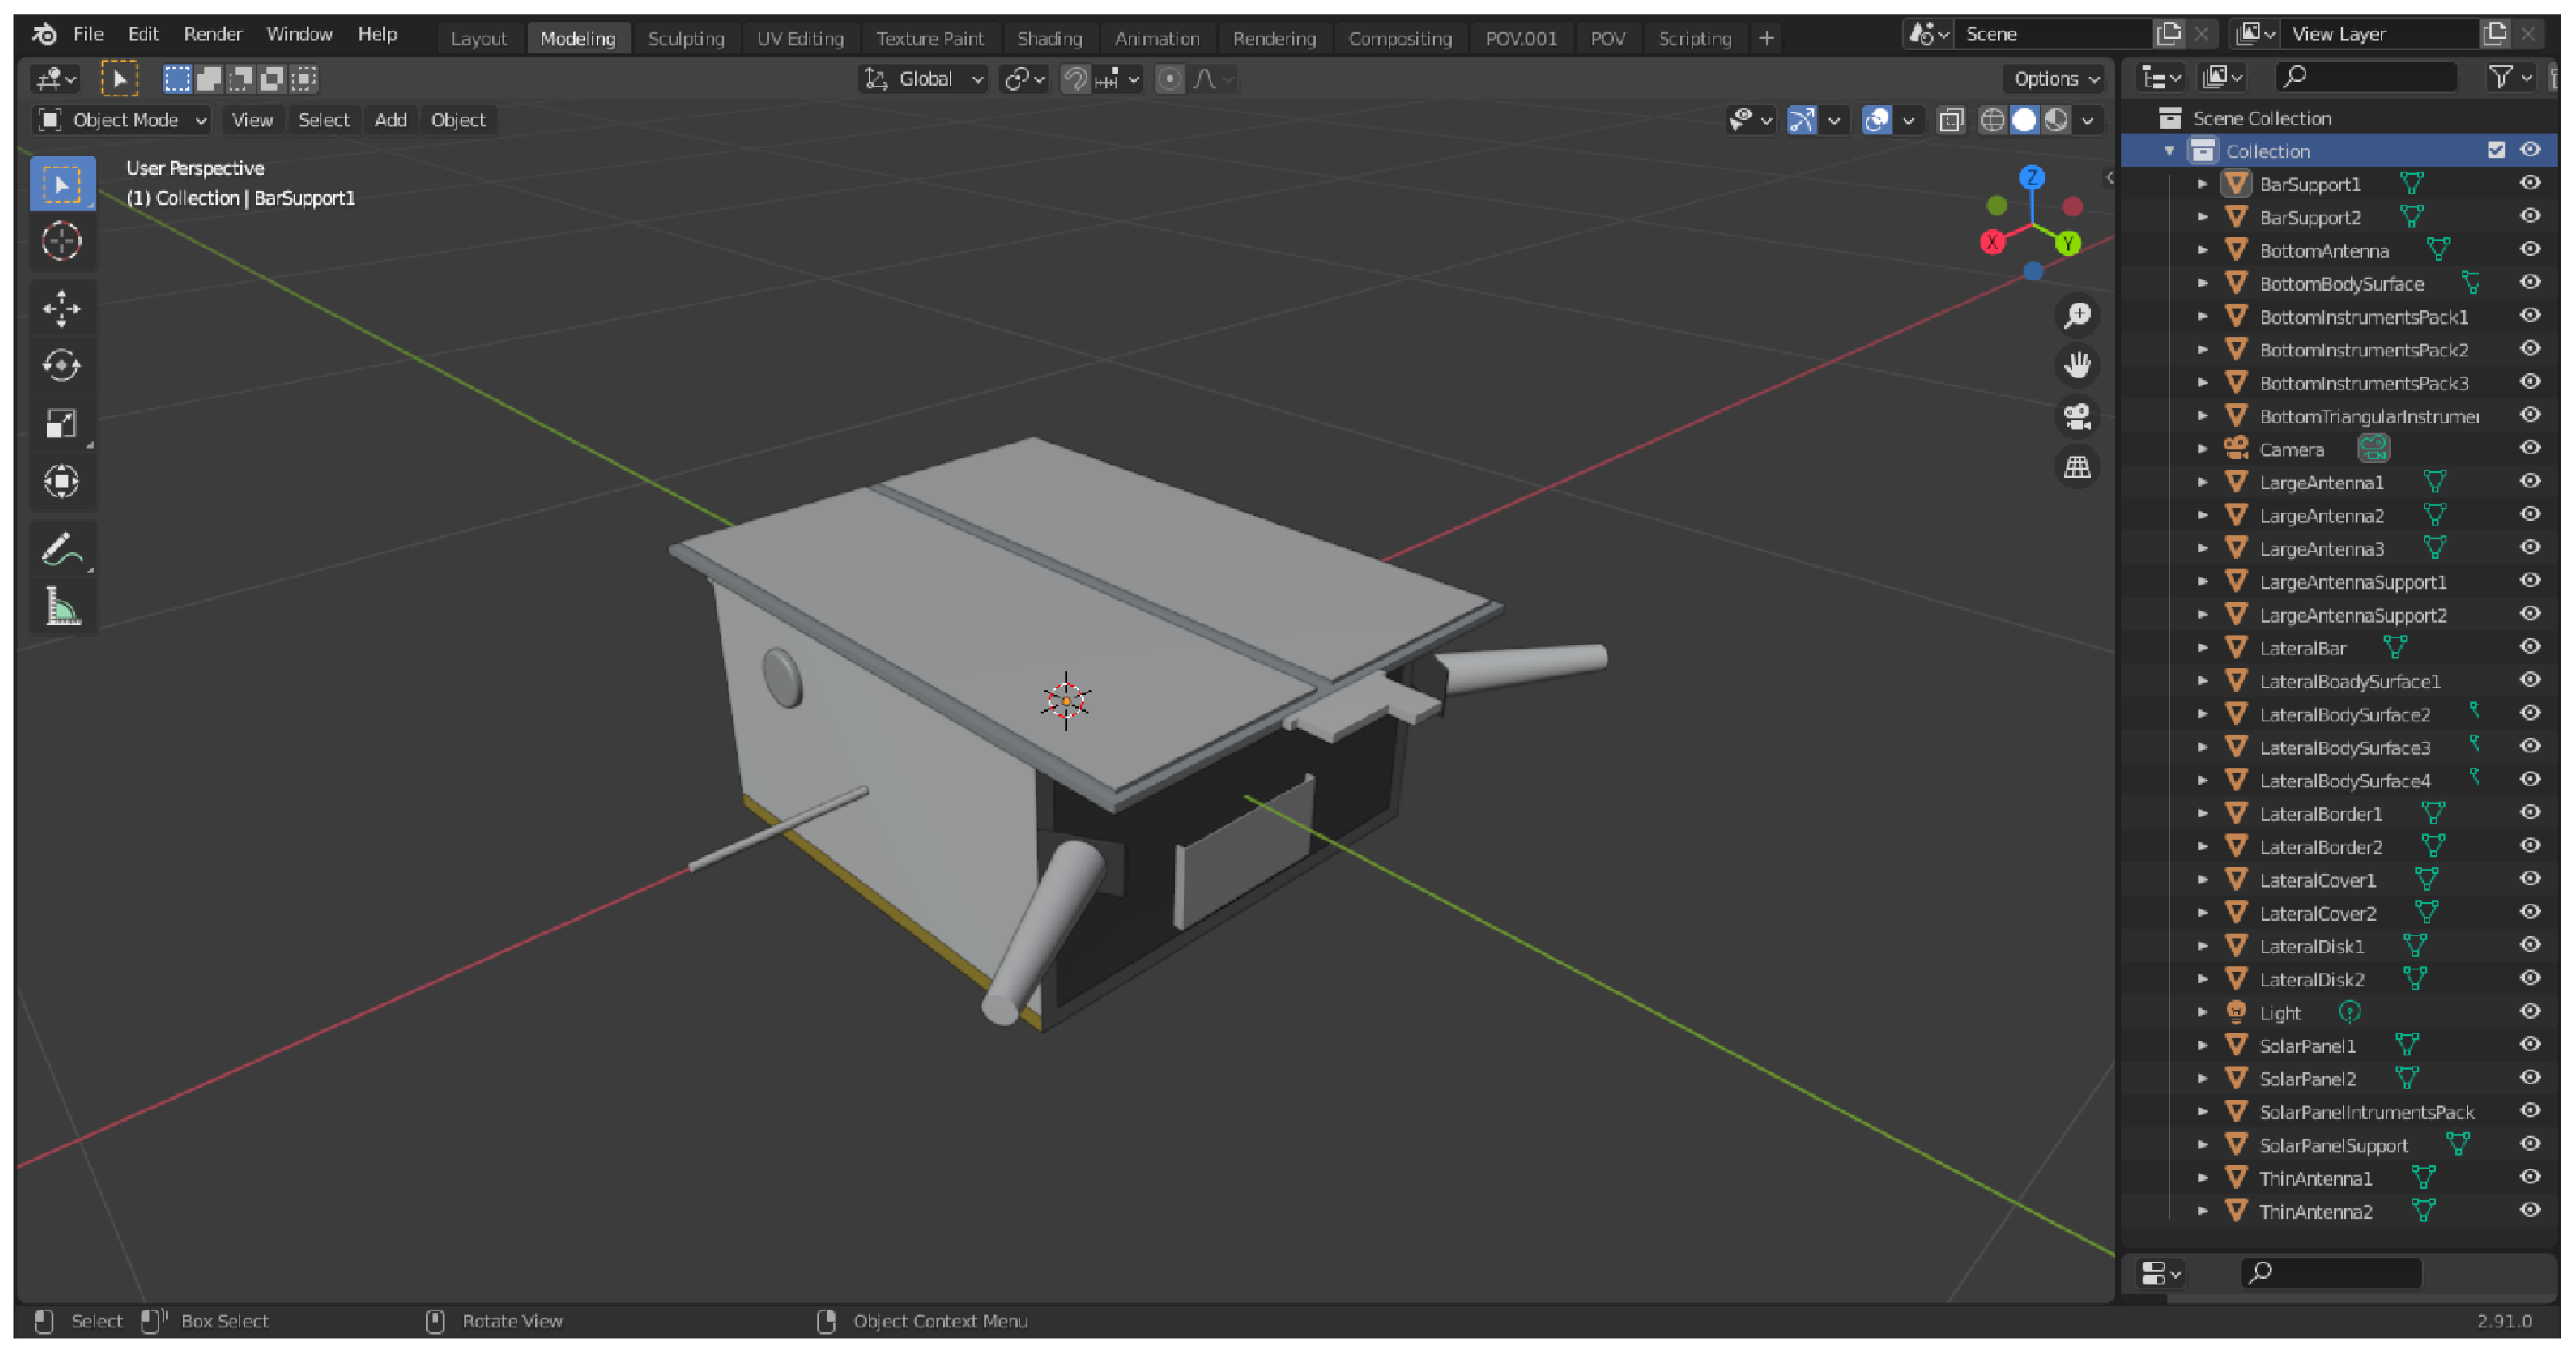
\includegraphics[width=0.82\textwidth]{gfx/tangoBlender.eps}
  \caption{Tango \acrshort{sc} \acrshort{3d} model in Blender}
  \label{fig:tangoblender}
\end{figure}

The Blender \acrshort{povray} add-on also let the user to inject custom POV code (figure \ref{fig:tangoblenderpov}) into the auto-generated one, which can be useful especially for adding textures, for example to the solar panels.

\begin{figure}[htbp]
  \centering
  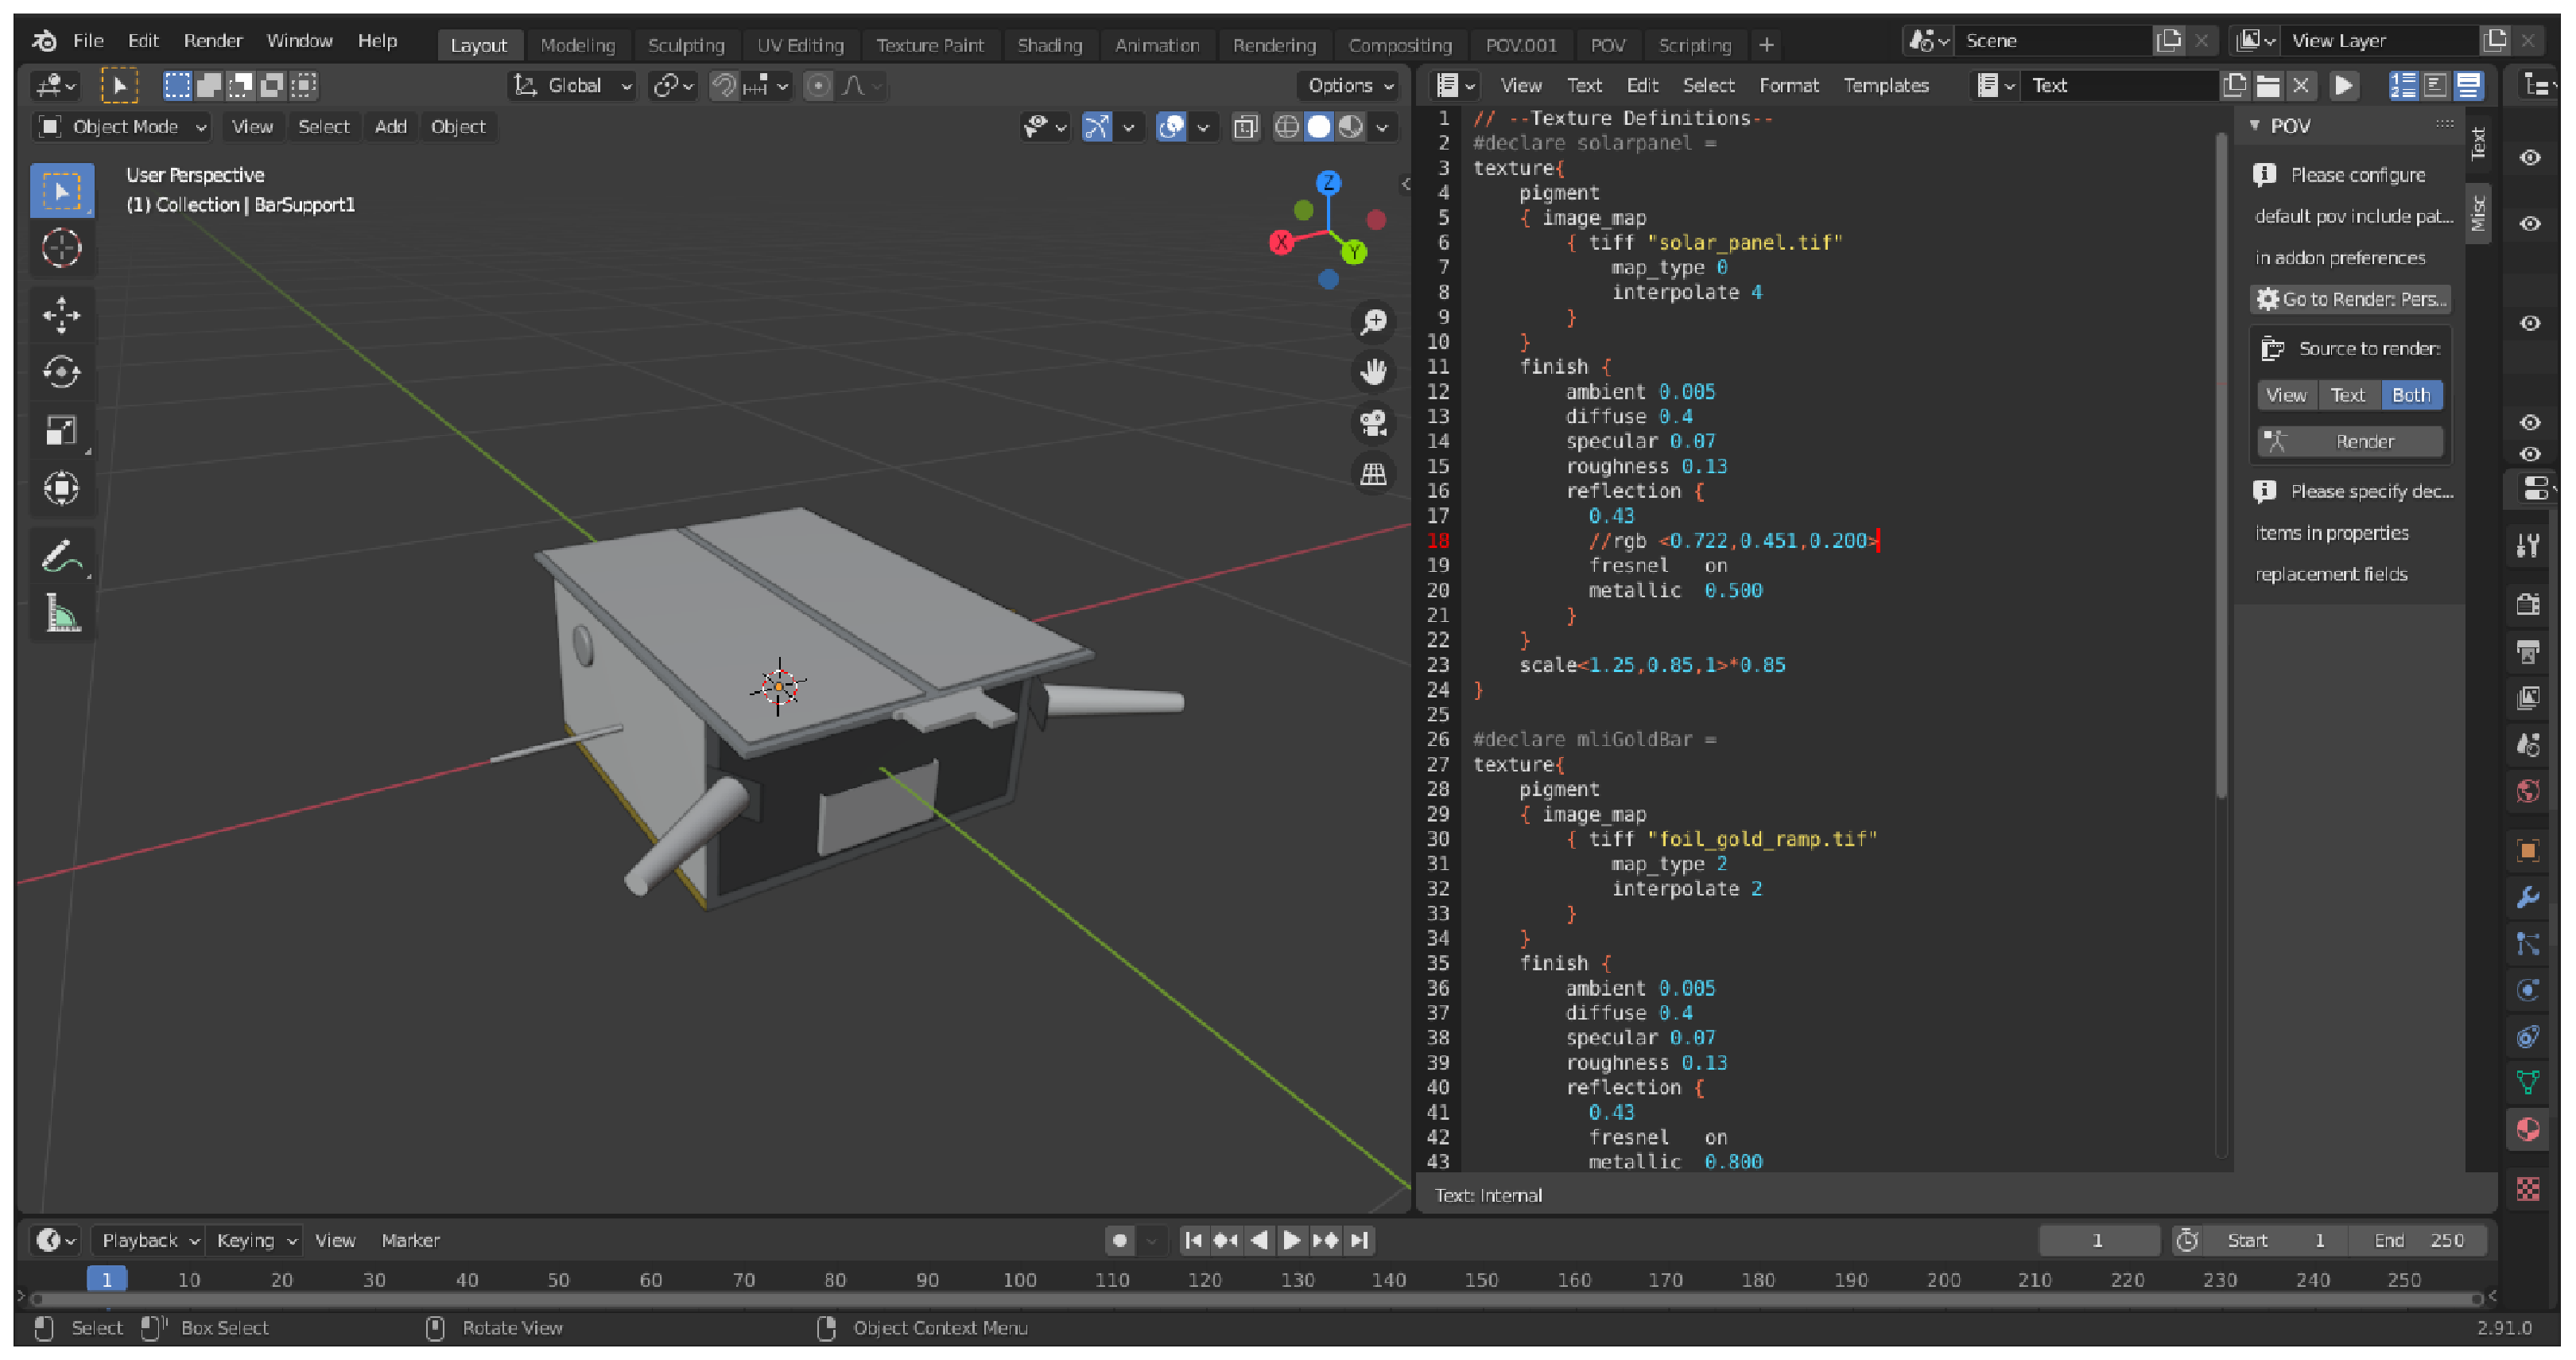
\includegraphics[width=0.82\textwidth]{gfx/tangoBenderPOVCode.eps}
  \caption{Add custom POV code into Blender}
  \label{fig:tangoblenderpov}
\end{figure}

\begin{figure}[htbp]
  \centering
  
\includegraphics[width=0.45\textwidth]{gfx/foil_gold_ramp.eps}
  \caption{Texture used to model MLI}
  \label{fig:mliTexture}
\end{figure}

\begin{figure}[htbp]
  \centering
  \includegraphics[width=0.45\textwidth]{gfx/solar_panel.eps}
  \caption{Texture used to model solar panels}
  \label{fig:solarPanelTexture}
\end{figure}

The end results is showed in figure \ref{fig:tangoblenderfinal}

\begin{figure}[htbp]
  \centering
  \includegraphics[width=0.82\textwidth]{gfx/tangoPolished.eps}
  \caption{Tango \acrshort{sc} rendered using \acrshort{povray} Blender add-on}
  \label{fig:tangoblenderfinal}
\end{figure}

\subsubsection{\acrshort{povray}}
The major issue of the code generated from the  \acrshort{povray} Blender add-on is that is composed of several separated \textbf{mesh2} objects which makes almost impossible to rotate the whole object by imposing a given attitude matrix, since one is supposed to rotate all the \textbf{mesh2} objects by hand.\\
In order to workaround this limitation, from all the \textbf{mesh2} objects which have been generated from \acrshort{povray} Blender add-on are merged into one single \inlinecode{POV}{merge} object.
The \inlinecode{POV}{merge} \acrshort{povray} operation allows to bind two or more shapes into a single entity that can be manipulated as a single object, which is exactly what we want. The new object created by the merge operation can be scaled, translated and rotated as a single shape. The entire merge can share a single texture and optical parameters but each object contained in the union may also have its own texture and optical parameters, which will override any texture statements in the parent object. So, all the \textbf{mesh2} objects which are describing the \acrshort{sc} surfaces are merged into a single big (21K \acrshort{loc}) \textbf{spacecraft} \inlinecode{POV}{merge} object.
To ease the usage of the \inlinecode{POV}{merge} object, a \acrshort{povray} include file it is created, with the sole purpose of containing the \textbf{spacecraft} \inlinecode{POV}{merge} object.
The include file is read in as if it were inserted at that point in the file. Using include is almost the same as cutting and pasting the entire contents of this file into the scene. This allow to define the \textbf{spacecraft} \inlinecode{POV}{merge} once and call it from any other POV file just like any other predefined object is called, and so, it is possible to manipulate its position and orientation in a much more easier way by just using the \inlinecode{POV}{matrix} keyword. The \inlinecode{POV}{matrix} keyword  allows to specify directly the orientation of the \textbf{spacecraft} object, \gls{A_TN}, and its location with respect to \acrshort{povray} "inertial" world.
In table \ref{tab:SCParameters} are briefly resumed the optical parameters used to model the different part of the \acrshort{sc}.

\begin{table}[htbp]
  \centering
  \begin{tabular}{c cccc}
    \hline
    \hline
               & Solar Panels & Antennas  & Main Body \\
    \hline
    Ambient    & 0.0          & 0.25      & 0.25      \\
    Roughness  & 0.13         & 0.0005    & 0.0005    \\
    Brillance  & -            & 3.15      & 3.15      \\
    Diffuse    & 0.3          & 0.95      & 0.99      \\
    Reflection & {0.23, 0.5}  & {0.65, 1} & {0.65, 1} \\
    Specular   & 0.04         & 0.96      & 0.96      \\
    Phong      & -            & 0.43      & 0.43      \\
    Phong Size & -            & 25        & 25        \\
    \hline
    \hline
  \end{tabular}
  \caption{Optical parameters of \acrshort{sc} different parts}
  \label{tab:SCParameters}
\end{table}

\subsection{Camera Modeling}
\acrshort{povray} allows to simulate a perspective pinhole camera (more details about the pinhole camera will be given in section \ref{subsection:pinhole}). In \acrshort{povray}'s camera environment, the programmer can set all relevant camera parameters, which will be then used to simulate the camera trough which the scene will be rendered.
The most meaningful parameters which can be imposed are the location of the camera itself, the direction of the boresight axis (where is the camera looking at), the view angle and the direction of the camera reference frame.\\
The major issue which has been faced when modeling the camera in \acrshort{povray} is the fact that the program defaults to a left handed coordinate system to describe the scene, while all other software (like Autodesk Inventor, Blender) are using a right handed coordinate system.

\begin{figure}[htbp]
  \centering
  \subfloat[\acrshort{povray} axis directions]{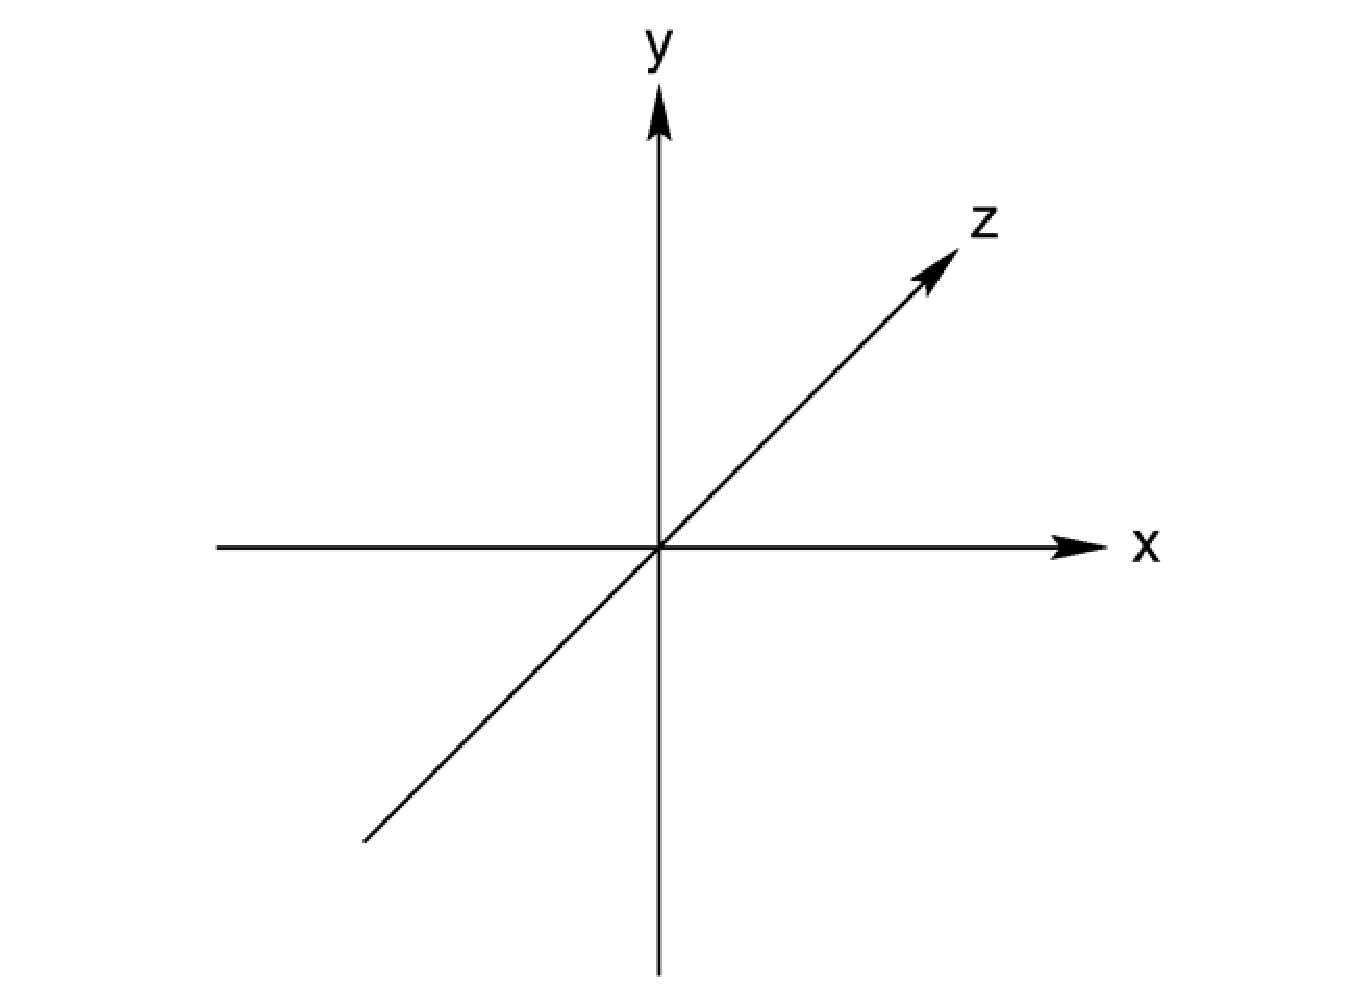
\includegraphics[width=0.4\textwidth]{gfx/povrayTern.eps}}
  \qquad
  \subfloat[Left hand rule]{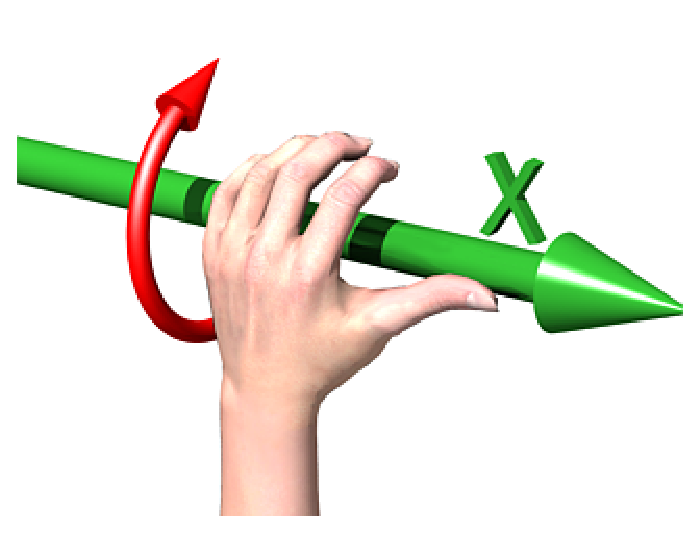
\includegraphics[width=0.4\textwidth]{gfx/povrayHand.eps}}
  \caption{\acrshort{povray} coordinate system}
  \label{fig:povraycoordinatesystem}
\end{figure}

Moreover, the right handed coordinate system is used also to model the orbit that the spacecraft will follow and the spacecraft attitude from Euler equations.
It is possible to trick \acrshort{povray} to behave like it using a right handed coordinate system by acting on the \inlinecode{POV}{right} vector of the camera environment. The camera \inlinecode{POV}{right} vector describes the direction to the right of the camera, so, in practicte, tells \acrshort{povray} where the right side of the screen is. Therefore, the  sign of the x component of the \inlinecode{POV}{right} vector can be used to determine the handedness of the coordinate system in use.

\begin{figure}[htbp]
  \centering
  \subfloat[Left Handed Coordinate System]{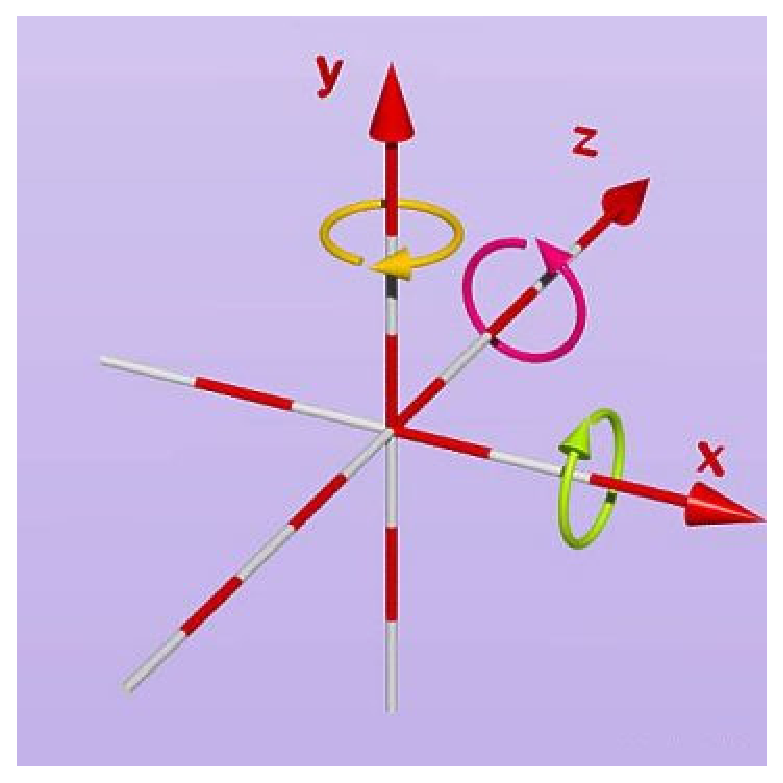
\includegraphics[width=0.4\textwidth]{gfx/axesLeft.eps}}
  \qquad
  \subfloat[Right Handed Coordinate System]{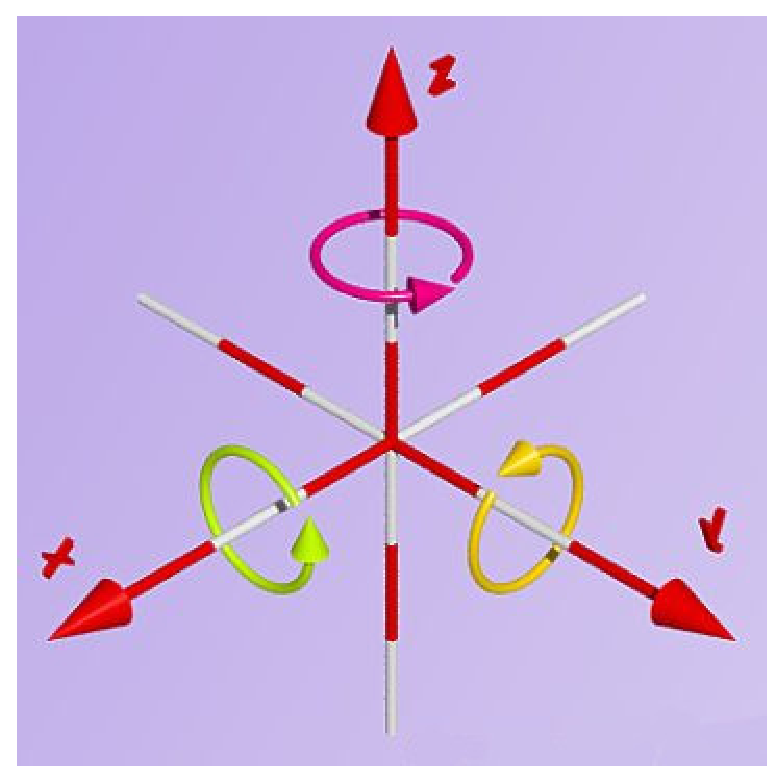
\includegraphics[width=0.4\textwidth]{gfx/axesRight.eps}}
  \caption{Left Handed Coordinate System and Right Handed Coordinate System}
  \label{fig:frames}
\end{figure}

By default \acrshort{povray} use a positive x value in the \inlinecode{POV}{right} vector. This means that the right side of the screen is aligned with the +x-direction. By using a negative x value in the \inlinecode{POV}{right} vector instead the right side of the screen will be aligned to the -x-direction, and the coordinate system will be right handed. Doing only that however left us having the y axis as the one pointing upward and the z axis as the one point in the direction which goes outside the screen.
To have a more comfortable reference frame, aligned with the \acrshort{gci} reference frame introduced in section \ref{sec:refereceFrames}, we can flip y and z axis by overriding the \inlinecode{POV}{sky} vector. By default, in fact, \acrshort{povray} uses \inlinecode{POV}{<0,1,0>} as \inlinecode{POV}{sky} vector. By redefining it as \inlinecode{POV}{<0,0,1>}  \acrshort{povray} will roll the camera until the top of the camera is in line with the \inlinecode{POV}{sky} vector, giving us the desired reference frame.

\begin{figure}[htbp]
  \centering
  \subfloat[\acrshort{povray} standard coordinate system]{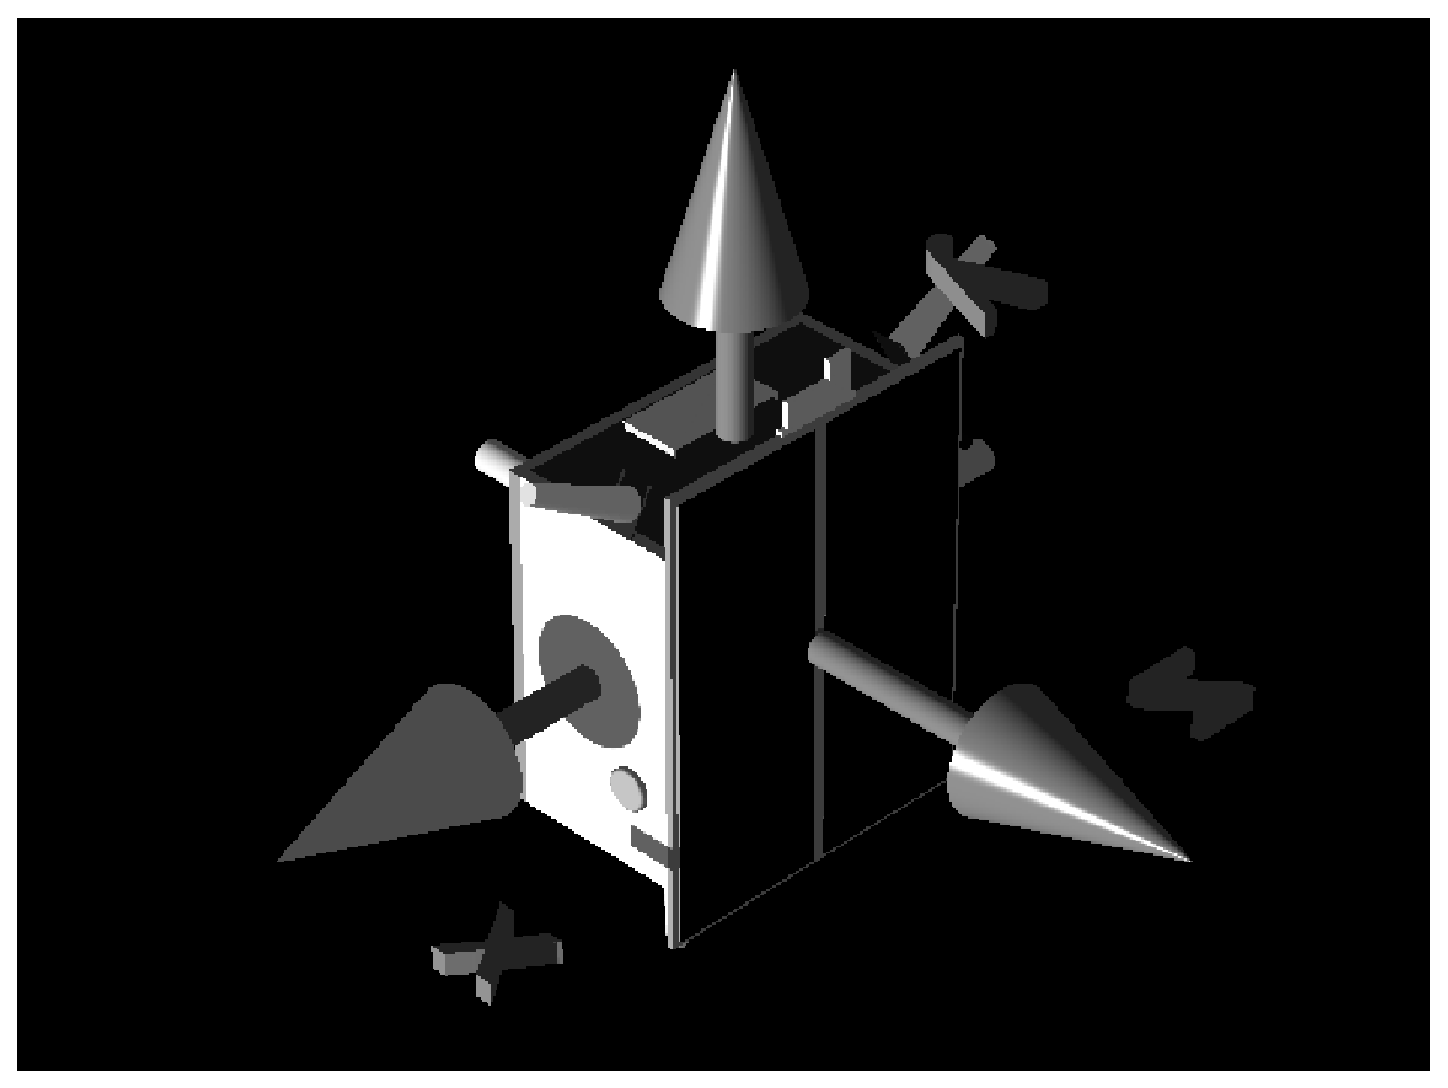
\includegraphics[width=0.47\textwidth]{gfx/tangoAxesNormal.eps}}
  \qquad
  \subfloat[Result after imposing negative x to the \inlinecode{POV}{right} vector ]{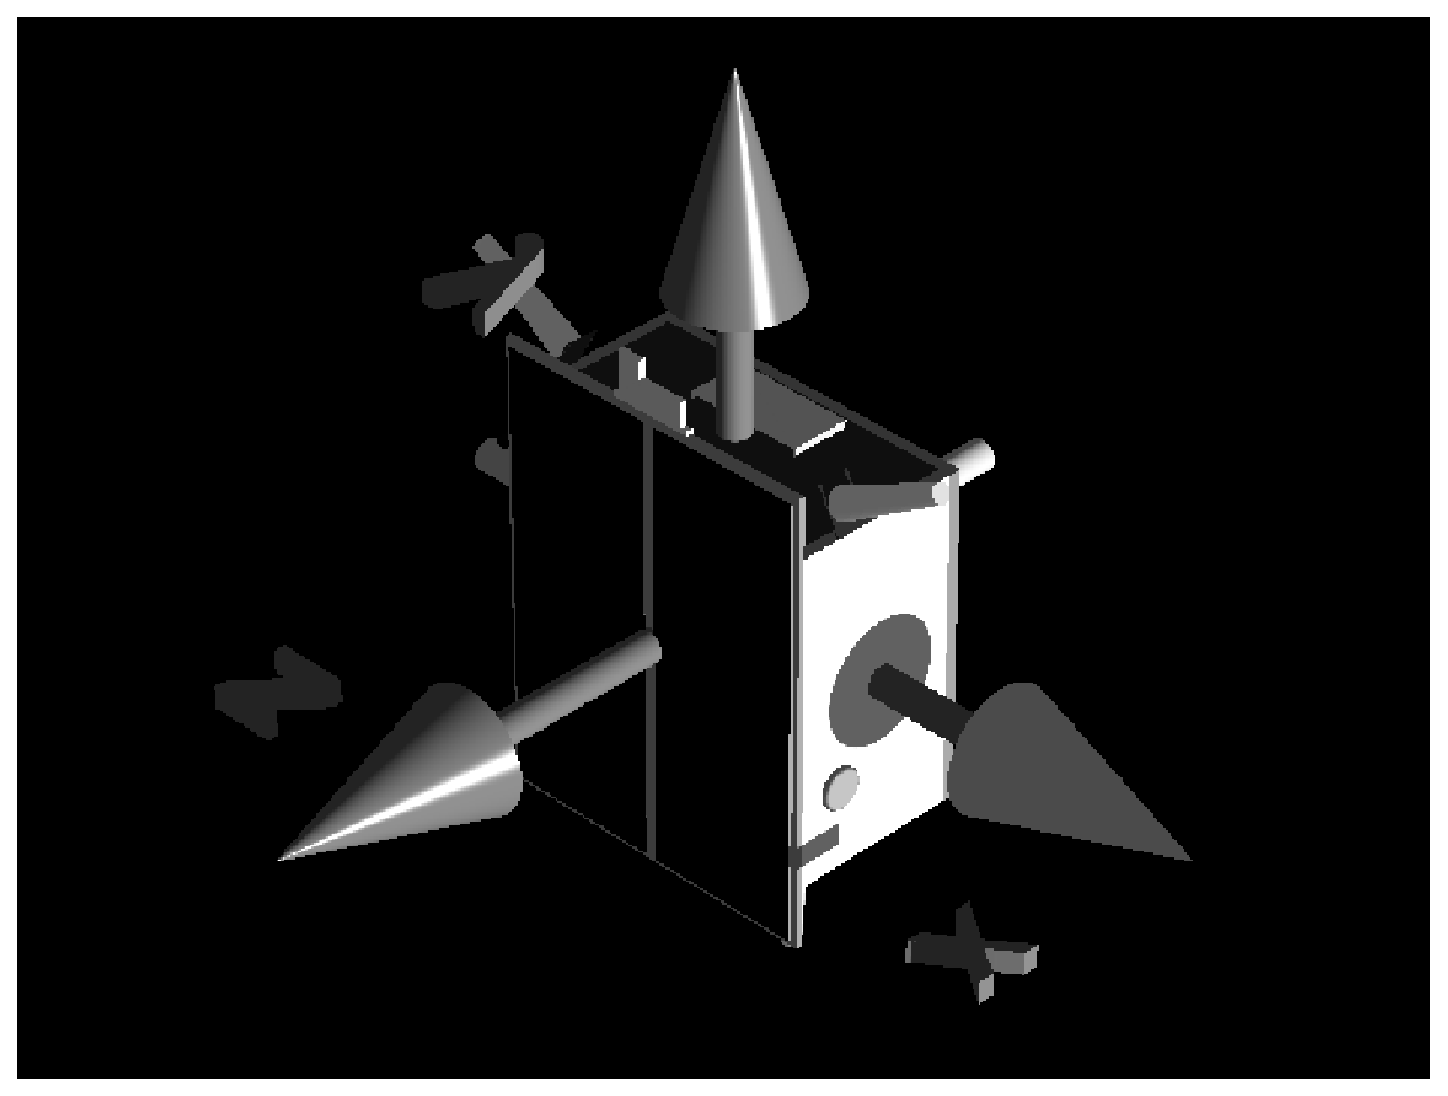
\includegraphics[width=0.47\textwidth]{gfx/tangoAxesAfterRight.eps}}
  \qquad
  \subfloat[Result after imposing \inlinecode{POV}{<0,0,1>} to the \inlinecode{POV}{sky} vector]{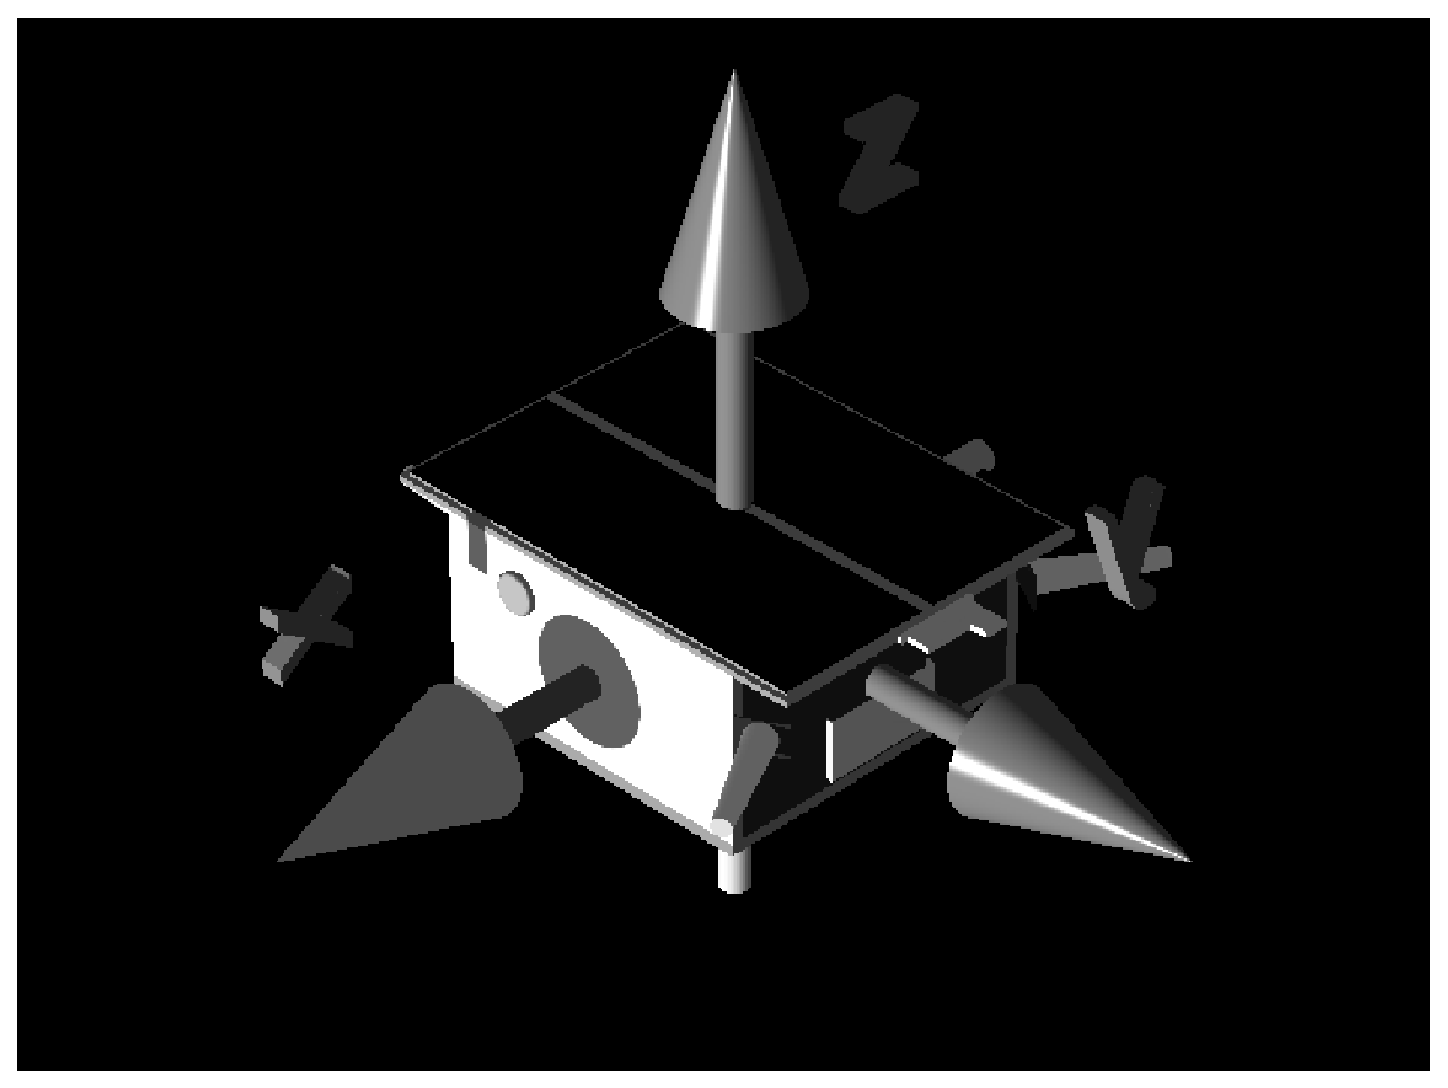
\includegraphics[width=0.47\textwidth]{gfx/tangoAxesSky.eps}}
  \caption{Reference Frame Rotations}
  \label{fig:framesComparison}
\end{figure}

In order to rightly simulate a real camera, the \acrshort{povray} camera aperture angle has been computed by assuming the intrinsic properties of a real camera, a Point Grey Grasshopper 3, equipped with a Xenoplan 1.9/17 mm lens, which is the same camera used to capture the real images of the SPEED data-set \cite{DBLP:journals/corr/abs-1911-02050}.

\begin{table}[htbp]
  \centering
  \begin{tabular}{ccc}
    \hline
    \hline
    Parameter & Description                 & Value             \\
    \hline
    $N_u$     & Number of horizontal pixels & 1920              \\
    \hline
    $N_v$     & Number of vertical pixels   & 1200              \\
    \hline
    $f_x$     & Horizontal focal length     & \SI{17.6}{\mm}    \\
    \hline
    $f_y$     & Vertical focal length       & \SI{17.6}{\mm}    \\
    \hline
    $d_u$     & Horizontal pixel length     & \SI{5.86e-3}{\mm} \\
    \hline
    $d_v$     & Vertical pixel length       & \SI{5.86e-3}{\mm} \\
    \hline
    \hline
  \end{tabular}
  \caption{Parameters of the camera used to capture the SPEED images \cite{DBLP:journals/corr/abs-1911-02050}}
  \label{tab:SPEEDCameraParameters}
\end{table}

By assuming a square \acrshort{ccd} sensor with square pixels we can obtain:

\begin{equation}
  A. R. = \frac{N_u}{N_v} \,,
\end{equation}

\begin{equation}
  CCD_{size} = d_u \cdot N_u \,,
\end{equation}

\begin{equation}
  \alpha = 2 \cdot \arctan{\left( \frac{CCD_{size}}{2 \cdot f_x} \right)} \,,
\end{equation}

where $A.R.$ is the Aspect Ratio of the picture, which is passed as first component \inlinecode{POV}{right} vector (with the negative sign, as described before), and $\alpha$ is the aperture angle which will be input in \acrshort{povray}.
Using the parameters detailed in table \ref{tab:SPEEDCameraParameters} we can compute:
\begin{itemize}
  \item \gls{ar} = $1.6$;
  \item \gls{alpha} = $35.4 ^{\circ}$.
\end{itemize}

\begin{figure}[htbp]
  \centering
  
\includegraphics[width=0.82\textwidth]{gfx/tangoNoNoise.eps}
  \caption{Tango \acrshort{sc} rendered using table \ref{tab:SPEEDCameraParameters} parameters}
  \label{fig:tangoNoNoise}
\end{figure}

\paragraph{Camera Attitude}\mbox{}\\
Being able to correctly know the imposed camera attitude at the moment of image generation is of crucial importance, especially when developing images to test pose determination algorithms.
Using the \inlinecode{POV}{look_at} keyword we specify the direction of the camera's boresight axis (so, in practice, where the camera is looking at, as the keyword itself suggest). Therfore, by imposing the \inlinecode{POV}{look_at} vector, we are implicitly imposing the camera attitude with respect to what is looking at. For what concerns this work, it is assumed that the camera always looks at the center of the target \acrshort{sc}.
By imposing \inlinecode{POV}{sky} and \inlinecode{POV}{right} vectors we impose the initial direction which \acrshort{povray} uses for orienting the camera.
By imposing the \inlinecode{POV}{look_at} vector \acrshort{povray} will first roll the camera until the top of the camera is in line with the sky vector. Then it uses the \inlinecode{POV}{sky} vector as the axis of rotation left or right and then to tilt up or down in line with the \inlinecode{POV}{sky} until until it lines up with the \inlinecode{POV}{look_at} point. Then tilts straight up or down until the \inlinecode{POV}{look_at} point is met exactly.

\begin{figure}[htbp]
  \centering
  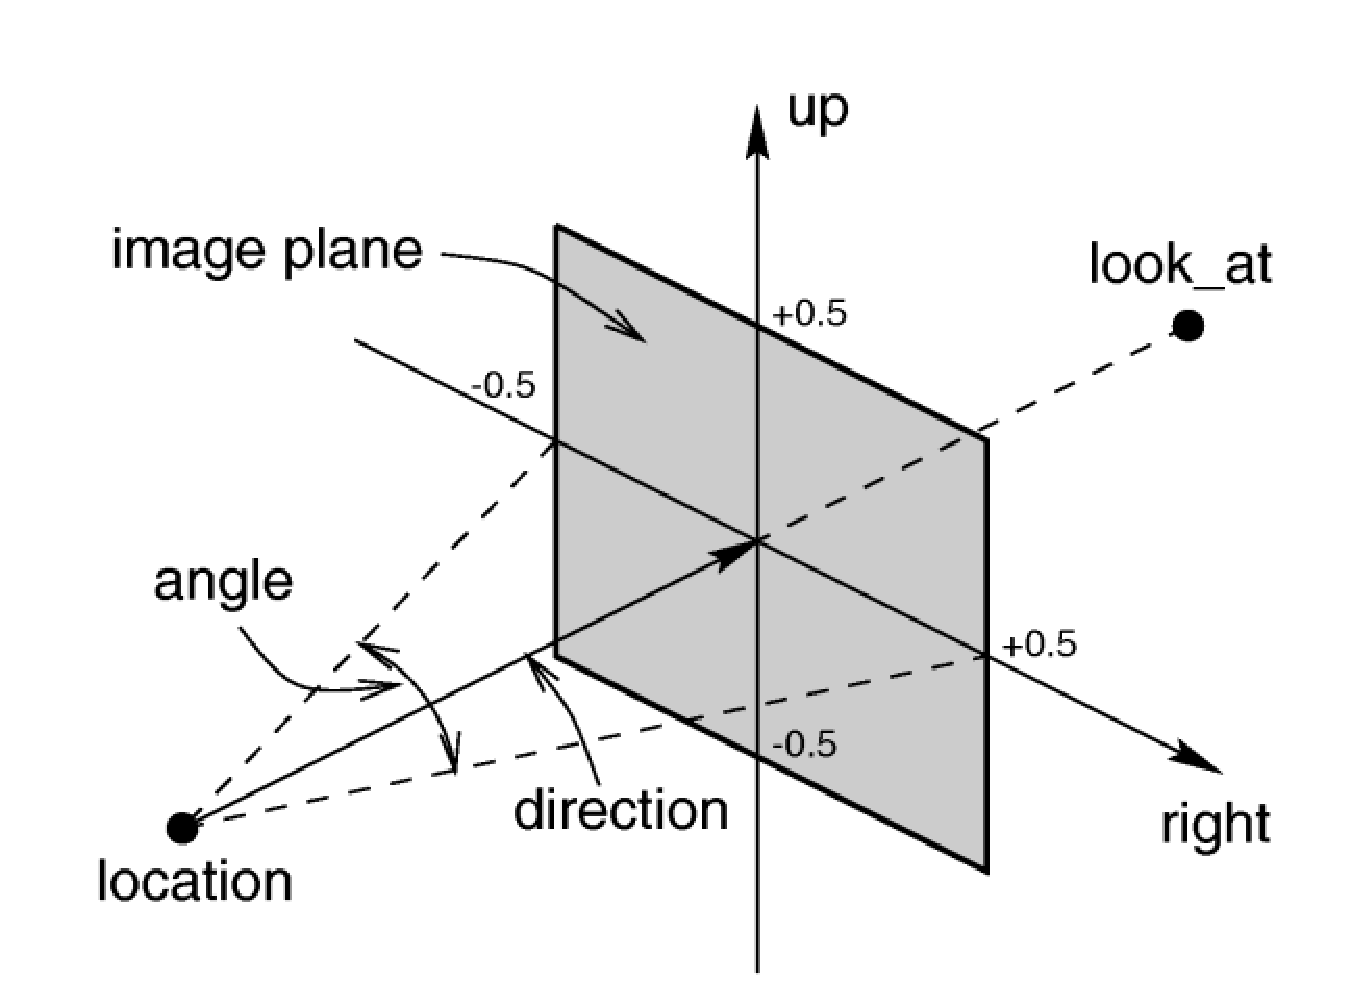
\includegraphics[width=0.82\textwidth]{gfx/perspcam.eps}
  \caption{\acrshort{povray} default perspective camera}
  \label{fig:perspcam}
\end{figure}

So, by knowing how \acrshort{povray} rotates the camera to point to the the \inlinecode{POV}{look_at} point, we can compute the actual attitude matrix of the camera with respect to the \acrshort{gci} frame\footnote{It is reminded to the reader that the \acrshort{gci} reference frame and the \acrshort{povray}'s world frame are aligned by design} exploiting simple linear algebra rules:

\begin{itemize}
  \item the z-direction, which is the one going straight out from the camera, can be computed by simply making the difference between the \inlinecode{POV}{look_at} vector and the camera \inlinecode{POV}{location} vector;
  \item the x direction, the one going right on the image plane, can be found by the cross product between the z-direction and the \inlinecode{POV}{sky} vector;
  \item the y direction, which is the one going downward in the image plane, can be found by performing the cross product between the z-direction and y-direction.
\end{itemize}

So, doing the needful math it is possible to write:

\begin{equation}
  \mathbf{\hat{z}} = \frac{\text{\inlinecode{POV}{look_at}} - \text{\inlinecode{POV}{location}}}{\norm{\text{\inlinecode{POV}{look_at}} - \text{\inlinecode{POV}{location}}}} \,,
\end{equation}

\begin{equation}
  \mathbf{\hat{x}} = \frac{\mathbf{\hat{z}} \wedge \text{\inlinecode{POV}{sky}}}{\norm{\mathbf{\hat{z}} \wedge \text{\inlinecode{POV}{sky}}}} \,,
\end{equation}

\begin{equation}
  \mathbf{\hat{y}} = \frac{\mathbf{\hat{z}} \wedge \mathbf{\hat{x}}}{\norm{\mathbf{\hat{z}} \wedge \mathbf{\hat{x}}}} \,.
\end{equation}

Knowing the versors which define the reference frame, the attitude of the camera with respect to the inertial \acrshort{povray} frame, \gls{A_CN}, can be simply defined as :

\begin{equation}
  \mathbf{{A_{CN}}} \triangleq [\mathbf{\hat{x}}, \mathbf{\hat{y}} \,. \mathbf{\hat{z}}]
\end{equation}

At this point, the imposed ground truth pose (\gls{A_TC}, \gls{t_c}) of the camera with respect to the \acrshort{sc} is completely defined by:

\begin{equation}
  \mathbf{{A_{TC}}} = \mathbf{{A_{CN}}} \mathbf{{A^T_{TN}}} \,,
\end{equation}

\begin{equation}
  \mathbf{t_C} = - (\text{\inlinecode{POV}{look_at}} - \text{\inlinecode{POV}{location}}) \mathbf{{A^T_{TN}}} \,.
\end{equation}

\subsection{Noise modeling}\label{subsection:addingthenoise}
Finally, for augmenting the "realness" of an image generated though \acrshort{povray}, the image needs to be post-processed using MATLAB.
The image so is input in MATLAB and two different noises are applied through the \inlinecode{MATLAB}{imnoise} command : speckle noise ($\sigma^2 = 0.004$) and Gaussian white noise ($\sigma^2 = 0.003$).
The final result can be seen in figure \ref{fig:comparisonNoise}.

\begin{figure}[htbp]
  \centering
  \subfloat[Image without noise added]{
\includegraphics[width=0.47\textwidth]{gfx/tangoNoNoise.eps}}
  \qquad
  \subfloat[Image wit speckle and Gaussian white noise]{\includegraphics[width=0.47\textwidth]{gfx/tangoNoise.eps}}
  \caption{Comparison between image without noise and image with speckle and Gaussian white noise}
  \label{fig:comparisonNoise}
\end{figure}

\section{MATLAB integration}
Since it would be highly unpractical to hand edit every time all the parameters to render the \acrshort{sc} in different position and attitudes as well as Earth's different rotations, a MATLAB toolbox has been developed which allows the user to automatically generate .pov \acrshort{sdl} files, and it renders them trough \acrshort{povray} automatically.
The implemented toolbox takes as input \gls{N_u}, \gls{N_v}, \gls{fx}, \gls{fy}, \gls{d_u}, \gls{d_v} to compute intrinsic camera parameters to set \acrshort{povray} camera.
Then, it offers the user the possibility to generate a sequence of random attitudes \cite{Arvo92}, given the orbital parameters of a reference orbit. If inertial properties of the target \acrshort{sc} are available, instead, it can compute the full uncontrolled dynamics (so to speak, the dynamics of the \acrshort{sc} when only subjected to the disturbances torques acting on the reference orbit) of the \acrshort{sc} trough a Simulink model at each time instant. For the interested reader, details about how the Space environment has been modeled in Simulink are given in \ref{app:first-appendix}.
For each time instant for which the attitudes of the target \acrshort{sc} have been computed, the relative position of the camera with respect to the target \acrshort{sc} is computed by selecting a random point inside a sphere having a \SI{20}{\m} radius centered in the target position, and the imposed pose is computed. A random Earth's rotation is computed as well.
All the properties of the scene are stored in a custom .att file, which can be passed in a second time to retrieve the absolute position and orientation of both the camera and the target \acrshort{sc} and their pose.
A .pov \acrshort{sdl} file is written for each time instant for which the attitudes of the target \acrshort{sc} have been computed and \acrshort{povray} is called to render each image in the background, from within MATLAB. Rightly after an image has been rendered, it is post-processed by MATLAB in order to add the noise, as described in \ref{subsection:addingthenoise}.

\section{Conclusions}
It must be noted by the reader, that a patched \acrshort{povray} version is required in order to correctly replicate what has been done in this project, as stated in the first lines of section \ref{sec:3dmodel}. At the beginning of this project it has been decided that by design, 1 unit in the \acrshort{povray} world is exactly equal to \SI{1}{\km} to ease the modeling of the solar system. Thus, the Earth is placed at the origin of the \acrshort{povray} world (consistently with the \acrshort{gci} frame)and it has a \SI{6378}{\km} radius, and the light source, the Sun, is placed \SI{1.4723e8}{\km} far from the Earth, and has a radius of \SI{696340}{\km}.
The \acrshort{sc} instead is placed on an orbit characterized by the orbital parameters specified in table \ref{tab:orbitalParameters}. The inertial properties of the target instead are computed by assuming a mass of \SI{50}{\kg} and using the dimension given in \ref{sec:3dmodel}.

\begin{table}[htbp]
  \centering
  \begin{tabular}{ccc}
    \hline
    \hline
    Orbital Parameters & Symbol   & Values         \\
    \hline
    Apogee             & $r_a$    & \SI{7178}{\km} \\
    \hline
    Perigee            & $r_p$    & \SI{7101}{\km} \\
    \hline
    Semimajor axis     & $a$      & \SI{7133}{\km} \\
    \hline
    Inclination        & $i$      & \ang{98.28}    \\
    \hline
    Pericenter anomaly & $\omega$ & \ang{0}        \\
    \hline
    True anomaly       & $\theta$ & \ang{0}        \\
    \hline
    Eccentricity       & $e$      & \ang{0.0045}   \\
    \hline
    \hline
  \end{tabular}
  \caption{Parameters used to generate the reference orbit \cite{prismaOrbitParameters}}
  \label{tab:orbitalParameters}
\end{table}

So, what is being represented is a scene having an extremely small object (the \acrshort{sc}) in front of a giant object {the Earth}, which is impacted by light which is generated from a very far distance (the Sun). Due to the exquisite peculiarity of this kind of scene, in some corner cases a "bounding issue" can be triggered, causing the \acrshort{sc} to be only partially redendered in the scene, or, in worst case scenario, not being rendered at all. Directly citing the \acrshort{povray} documentation, in order to speed up the ray-object intersection tests \acrshort{povray} uses a variety of spatial sub-division systems. The primary system uses a hierarchy of nested bounding boxes. This system compartmentalizes all finite objects in a scene into invisible rectangular boxes that are arranged in a tree-like hierarchy. Before testing the objects within the bounding boxes the tree is descended and only those objects are tested whose bounds are hit by a ray. This can greatly improve rendering speed. However, during the development of this project turned out that \acrshort{povray} automatic bounding is not perfect. There are situations where a perfect automatic bounding is very hard to calculate, like the one faced in this project. Unfortunately, \acrshort{povray} developers removed the possibility of turning off bounding control in \acrshort{povray}, thus it is necessary to compile a patched \acrshort{povray} version which introduces back the command line switch \textbf{-MB} which allows the user to turn off bounding control. According to the GPL license \acrshort{povray} is shipped with, the patch has been made freely available \footnote{\url{https://github.com/fcuzzocrea/povray/commit/2aecdfb20eef3ed3b6a5698392a9c91fa3f1afcd}}.
The output of the toolbox which has been described trough this chapter can be observed in figure \ref{fig:finalResult}.

\begin{figure}[htbp]
  \centering
  \subfloat[]{\includegraphics[width=0.47\textwidth]{gfx/tango/tango_14.eps}}
  \qquad
  \subfloat[]{\includegraphics[width=0.47\textwidth]{gfx/tango/tango_15.eps}}
  \qquad
  \subfloat[]{\includegraphics[width=0.47\textwidth]{gfx/tango/tango_31.eps}}
  \qquad
  \subfloat[]{\includegraphics[width=0.47\textwidth]{gfx/tango/tango_60.eps}}
  \qquad
  \subfloat[]{\includegraphics[width=0.47\textwidth]{gfx/tango/tango_259.eps}}
  \qquad
  \subfloat[]{\includegraphics[width=0.47\textwidth]{gfx/tango/tango_268.eps}}
  \qquad
  \subfloat[]{\includegraphics[width=0.47\textwidth]{gfx/tango/tango_228.eps}}
  \qquad
  \subfloat[]{\includegraphics[width=0.47\textwidth]{gfx/tango/tango_258.eps}}
  \qquad
  \caption{Final result}
  \label{fig:finalResult}
\end{figure}